\documentclass{book}
%\usepackage{html} % for latex2html commands
\usepackage{amsmath}
\usepackage{amssymb}
\usepackage{appendix}
\usepackage{tikz}
\usepackage{verbatim}

\title{\bf Weenix}
% TODO replace with appropriate title page directives:
\author{Brown University Department of Computer Science \\ Authored by \textit{Operating Systems} Teaching Assistant Staff \\ Edited by Dan Kimmel and J. Rassi}

%
% links:
% define \wlink to abstract over \hyperref (html hyperref uses different syntax)
% note that "%begin{latexonly}" is a construct for latex2html, not a commented-out command
%

%begin{latexonly}
\usepackage{hyperref}
%end{latexonly}

%\begin{htmlonly}
%\newcommand{\wlink}[2]{\hyperref[hyper][#1]{#2}}
%\end{htmlonly}
%begin{latexonly}
\newcommand{\wlink}[2]{\hyperref[#1]{#2}}
%end{latexonly}

%begin{latexonly}
\hypersetup{colorlinks, linkcolor=gray, urlcolor=gray}
%end{latexonly}

%
% document body
%

\begin{document}
    \maketitle
    \tableofcontents
	\part{Introduction}
        \chapter{The Weenix OS}
\label{the-weenix-os}

\section{Motivation}


The Weenix operating system is a project for people interested in writing parts of a Unix kernel. The operating system was originally written in 1998 by teaching assistants for Brown University's operating systems course, taught by Professor Tom Doeppner, and has been maintained by that course's staff ever since. While the operating system is mostly based on early versions of Unix, it incorporates many recent developments in operating systems.
    
This book is intended to be a guide for students who are working on the Weenix operating system and those interested in contributing to it.
Part 1 is an introduction to Weenix, including the basics of setting up your development environment, using the build system, and running the OS in a virtual machine.
Part 2 contains five chapters, each of which specify an assignment. In the operating systems course taught at Brown, students have a choice between doing either:

\begin{itemize}
    \item All five assignments.
    \item A separate threads library assignment followed by two of the Weenix assignments (\wlink{vfs}{VFS} and \wlink{s5fs}{S5FS}).
\end{itemize}

Students pursuing the former option are assigned a mentor from the course staff who will be a source of clarification or hints if the student wishes. The latter option is provided to allow students who are not interested in a career in operating systems development to learn the basics of operating systems without spending the better part of their semester hacking the Weenix kernel. Each assignment chapter begins with an overview of the assignment, then describes the expected implementation in more detail, and ends with tips for testing.
Part 3 describes the inner workings of some key parts of the kernel not typically explored during the assignments. This is mainly a resource for those wishing to contribute to the Weenix project.
Finally, several appendices are included which provide more details about development tools, online resources, and the protocols of contributing new code.

\section{How to Read This Book}
We expect that there are at least two groups of people who will want to read this book. If you are someone who wants to see Weenix run \emph{right now}, jump ahead to \nameref{quickstart}. Everyone else should begin by reading \nameref{project-management} and then can read the assignments, manual, and appendices in whatever order they please. However, if you plan to do the assignments, we recommend that you do them in order, as they build on top of one another.

\section{History}
The Weenix OS, and the course that it grew up with, have a long and illustrious history. Although the Brown operating systems course has been taught since the 1960s, Weenix was first written in the spring of 1998, running on what was known only as the Brown Simulator 2.0. The two pieces of software were written by Keith Adams, Michael Castelle, Caroline Dahllof, Jason Lango, and Dave Powell. The name Weenix (``little *nix'') was invented by Keith Adams, and the OS was designed based on early versions of Unix. In 2004, a competing Brown operating system based on Windows (named HipOS) was created by Hari Khalsa, whose effort was apparently completely vanquished. During 2007-2009, Weenix moved off of the Brown Simulator and onto Xen virtual machines, an effort spearheaded by David Pacheco, Joel Weinberger, Dan Kuebrich, and Dimo Bounov. In 2010, Weenix found its current home running on Bochs, a virtual machine including a simulated real machine. Chris Siden, Alvin Kerber, and Shaun Verch were the major contributors for this move. Weenix has since moved onto QEMU, an x86 processor emulator.

The features of Weenix now include:
\begin{itemize}
    \item Intelligent multitasking
    \item Virtual memory
    \item Terminal emulation
    \item Polymorphic file system support
    \item Advanced device support (including APIC and PATA with BMIDE)
\end{itemize}

\section{Acknowledgements}
Weenix would not have been possible without the help of many earnest, devoted individuals. Thanks first to Professor Tom Doeppner, for his patient guidance and leadership.

Thanks also to the many course TAs since the creation of Weenix.
\begin{itemize}
    \item['98-'99] Mike Castelle, David Powell, Caroline Dahllof, Tim Rowley
    \item['99-'00] Thomas Crulli, Matt Eccleston, Keith Adams, Matt Ahrens, Tim Rowley
    \item['00-'01] Matt Ahrens, Adam Leventhal, Matt Amdur, Pete Demoreuille, Ioannis Tsochantaridis
    \item['01-'02] Pete Demoreuille, Peter Griess, Fareed Behmaram-Mosavat, Dan Polivy, Dmitriy Genzel
    \item['02-'03] Kit Colbert, Sean Cannella, Albert Huang, Eric Schrock, Mark Ture
    \item['03-'04] Susannah Raub, Dan Stowell, Luke Peng, Pat Sunday, David Reiss
    \item['04-'05] Mark Johnson, Stacy Wong, Sean Smith, Dan Spinosa, Hari Khalsa
    \item['05-'06] Lucia Ballard, Eric Tamura, Edwin Chang, Pat Culhane, Adam Fenn
    \item['06-'07] Dan Leventhal, Aaron Myers, Adam Cath, Dave Pacheco, Joel Weinberger
    \item['07-'08] Colin Gordon, Itay Neeman, Dan Kuebrich, Aurojit Panda, Lincoln Quirk, Owen Strain
    \item['08-'09] Andres Douglas, Tim O'Donnell, Dimitar Bounov, Brandon Diamond, Travis Fischer, Allan Shortlidge
    \item['09-'10] Spencer Brody, Robert Mustacchi, Chris Siden, Travis Webb
    \item['10-'11] Chris Siden, Venkatasubramanian Jayaraman, Alvin Kerber, Matt Mallozzi, Ryan Zelen
    \item['11-'12] Shaun Verch, Dan Kimmel, J. Rassi, Basil Crow, Irina	Calciu, Nickolay Ratchev, Andrew Ayer, Marcelo Martins
    \item['12-'13] Ethan Langevin, Aswin Karumbunathan, Jordan Place, Matt Krukowski, Dave Kilian, Irina Calciu
    \item['13-'14] Eric Caruso, Jackson Owens, James Kelley, Joel Nackman, Eli Wald, Zhixiong Chen
    \item['14-'15] DJ Hoffman, Ryan Roelke, Jake Ellis, Alex Kleiman, Alex Light, Indy Prentice, Eli Rosenthal
\end{itemize}
In particular, many thanks to Keith Adams, Adam Fenn, Dave Pacheco, Dimitar Bounov, Alvin Kerber, and Chris Siden for their major contributions to the project.

Finally, thanks to the innumerable students who have implemented Weenix over the years. We hope the knowledge you gained in the process has served you well.


        \chapter{Project Management}
\label{project-management}

\section{Introduction}

The first section of this chapter guides the reader through the process of producing a Weenix assignment from the project's complete source code (useful for course instructors), and the second explains how to set up a development environment for implementing the assignment yourself (useful for students).

\section{Preparing Weenix Assignments}

This section will walk you though a sample run of Weenix, and then shows you how to remove sections of code from the full implementation to allow you or your students to re-implement them.

\subsection{Quick Start: Getting Weenix Running} \label{quickstart}

See instructions in the top-level \texttt{README} file.

% \subsection{Environment}

\subsection{Getting the Source}
Requests for a copy of Weenix may be made via email to \texttt{weenix-devel@lists.cs.brown.edu}.
\subsection{Dependencies}
The following is required to run Weenix:

\begin{itemize}
\item \texttt{gcc}, the GNU C compiler % TODO what are the minimum version requirements for gcc/binutils?
\item \texttt{make}, the GNU build system
\item \texttt{qemu},% \textit{or} \texttt{bochs} \textit{or} \texttt{VirtualBox},
the processor emulator that Weenix runs on top of
\item \texttt{genisoimage} \textit{or} \texttt{mkisofs} (necessary to generate the disk image used by the emulator)
% \item \texttt{xorisso} and \texttt{grub-mkrescue} (necessary to generate the disk image used by the emulator)
\item \texttt{python}, at least 2.6 (but 2.x only)
\item \texttt{bash}
\end{itemize}

The following is optional, but recommended:
\begin{itemize}
\item \texttt{git}, the version control system
\item \texttt{gdb}, the GNU debugger, and \texttt{xterm} % TODO "Weenix includes special extensions to gdb writen using gdb's python extension api. In order to use these extensions you must be using at least gdb version 7.3"
\item \texttt{cscope} (for easier browsing of the Weenix source)
\end{itemize}

% TODO restore this section once bochs/vbox support is fixed in ./weenix
% For hardware virtualization, Weenix can use QEMU, Bochs, or VirtualBox.  We recommend QEMU, for its relative ease of setup and (we've found) superior simulation speed and quality.  You may need a special build of Bochs in order to use it with Weenix; feel free to contact \texttt{weenix-devel@lists.cs.brown.edu} if Weenix doesn't seem compatible with your installation of Bochs.

\subsection{Configuration}
Configuration for Weenix is available through editing the files \texttt{Config.mk} and \texttt{Global.mk}, which contain \texttt{VARIABLE=value} assignments in make syntax.  \texttt{Global.mk} contains directives relevant to the environment that Weenix is running in (e.g. alternative locations for utilities like \texttt{python} or \texttt{gdb}), while \texttt{Config.mk} is used to configure values that affect the behavior of Weenix itself (such as what modules to enable during the compilation process, or the size of the virtual disk to create).

In particular, you should be aware of the directives that affect what assignment to enable.  These are the first directives of \texttt{Config.mk}.  For example, to enable the S5FS assignment, set the first three to \texttt{1} (\texttt{DRIVERS=1}, \texttt{VFS=1}, and \texttt{S5FS=1}).

\subsection{Blanking Solutions}

This section will teach you how to blank the solution for individual assignments.  You will wish to do this before you attempt to complete the Weenix assignments (otherwise, you will find that they have already been done for you!) or before you assign them to others.

The script \texttt{make-weenix-repo.py} in the \texttt{tools/} directory performs this task.  It removes the contents of specially-marked functions, putting a \texttt{NOT\_YET\_IMPLEMENTED()} marker in their place.  It also initializes a fresh git repository in the root of the source tree for you (or your students) to clone from.

\begin{enumerate}

\item Obtain an unmodified copy of the Weenix source tree.

If you skip this step, you will lose all of your work: the \texttt{make-weenix-repo.py} will obliterate any git history that exists in the current source tree, as well as the contents of assignments that are to be removed.

\item Change into the \texttt{tools/} directory.

\item Run \texttt{./make-weenix-repo.py --cutextra all --cutsource [ASSIGNMENTS]}, where [ASSIGNMENTS] is a comma-delimited list of the projects you want to assign (or ``all'', without quotes).

For example, suppose you want to implement the S5FS and VM assignments.  You should blank the solutions for these assignments, and leave the rest (PROCS, DRIVERS, and VFS) intact.  This can be accomplished with the command:

\begin{verbatim}
$ ./make-weenix-repo.py --cutextra all --cutsource S5FS,VM\end{verbatim}

The order of the assignments is: PROCS, DRIVERS, VFS, S5FS, and lastly VM.  Remember that each assignment depends on its predecessor in order to run.  For example, if you wish to start with the VM assignment, do not blank any other assignments, or you will find yourself unable to run the VM code you write.

As another example, suppose you want start fresh from the first assignment.  Run:

\begin{verbatim}
$ ./make-weenix-repo.py --cutextra all --cutsource all\end{verbatim}

\item Update the assignment directives in \texttt{Config.mk} to reflect the first assignment you will work on.

These are described in detail in the Configuration section.

For example, if you are starting with the VFS assignment, set your assignment directives to:

\begin{verbatim}
DRIVERS=1
    VFS=1
   S5FS=0
     VM=0
DYNAMIC=0\end{verbatim}

If you are making use of the git repository, you will need to commit this change.  For example:

\begin{verbatim}
$ git commit -m 'Updated Config.mk assignments directives' Config.mk\end{verbatim}

\end{enumerate}

Congratulations: you are now ready to start the assignment.  If you need to distribute the assignment to others, have them copy (or \texttt{git clone}, if you are using git) this source tree to be their fresh copy to start working on.

\section{Implementing Weenix Assignments}

This section introduces some essential concepts in Weenix to e.g. a student who is interested in completing a Weenix assignment.

\subsection{A Message to the Reader}
Although this section is ostensibly about getting to know the Weenix codebase, we realize this is also the last part of the book we can be certain everyone will read, so we would like to give a few pieces of advice.

\begin{itemize}
    \item It is possible that this is your first exposure to a large code base. You should definitely spend some time poring over the existing code, thinking about what to implement. Take a look in Appendix \ref{LargeCodebases} to learn more about working in large codebases.
    \item For this and future assignments, it may be helpful to draw out a call graph (which functions call which) for the code you will be writing. Taking notes about the code as you read it is a useful skill for any codebase.
    \item Become an expert at using your chosen development tools. This will save you countless hours of time and energy, whether you learn to use a debugger (see Appendix \ref{Debugging}), text editor/IDE, cscope, version control, or something else. Many of these are mentioned in the appendix, so take a look there for some tips for getting started.
    \item Be sure to ask questions! The course staff is friendly and has a great working knowledge of the OS because they have implemented it themselves. Beyond that, getting Weenix working is far more rewarding if you understand \emph{why} something is done a particular way, and the repercussions of choosing a different way to do something.
    \item Take breaks to relax. \texttt{:-)}
\end{itemize}

\subsection{Build System}
The Weenix build system is based on the popular Unix utility \texttt{make}. It is meant to aid development by automating the compilation and linking of binaries, although it is used to automate several other things in the Weenix codebase as well.

In order to build the full operating system, \texttt{make} must be run in the top directory of the Weenix repository. Each \texttt{make} target corresponds to particular a set of commands listed in the \texttt{Makefile} located in the current directory. In the case of the top-level \texttt{Makefile}, \texttt{make all} simply descends into the \texttt{kernel} and \texttt{user} directories and executes \texttt{make} within each. The kernel and the userspace binaries can be built separately, by calling \texttt{make} from their respective directories. There are many different targets, such as individual object (\texttt{.o}) files, linked binaries and disk images, but the most useful targets are listed below.
  
To compile all the code using eight concurrent tasks, a user should run:
\begin{verbatim}
$ make -j 8 [all]\end{verbatim}
or potentially just:
\begin{verbatim}
$ make all
$ make       % defaults to target "all"\end{verbatim}
if the pretty output is more important than the speed of compilation.

Sometimes, such as after a change in the configuration settings or compiler flags, it is necessary to compile all the source code from scratch. However, \texttt{make} will only rebuild a file if it has been modified since the last time it was built. To delete all the constructed binaries and force \texttt{make} to compile from scratch, a user may run:
\begin{verbatim}
$ make clean; make all\end{verbatim}

\subsection{Assignment Specification}
To find out what to implement for a newly opened assignment, use the following command:
\begin{verbatim}
$ make nyi\end{verbatim}
This will produce a list of all the functions that are not yet written in the codebase with labels telling what file they are in and what assignment they are associated with.

Note that this command is only to be used with blanked assignments (otherwise, there's nothing to implement!).

\subsection{Running}
The \texttt{weenix} script has been provided for running the operating system inside a virtual machine or hardware simulator. It should be invoked from the topmost directory of the Weenix repository. To run it, one may simply use the command:
\begin{verbatim}
$ ./weenix\end{verbatim}

Until there is a functional on-disk file system, this is all that is necessary to run Weenix. However, at that point, the ability to create disks becomes very important. It is necessary to create a fresh disk the first time S5FS runs, and also after any time the disk is corrupted by a buggy kernel or unclean shutdown. The following command will run Weenix with a newly constructed disk:
\begin{verbatim}
$ ./weenix -n\end{verbatim}

At some point, it may be helpful to use a debugger to aid in the development of the operating system. The following command will begin Weenix in a virtual machine and attach \texttt{gdb} to it (if the virtual machine in use supports this option).
\begin{verbatim}
$ ./weenix -d gdb\end{verbatim}

%Finally, the script supports several different virtual machines and simulators.
%\begin{verbatim}
%$ ./weenix -m qemu   % the default
%$ ./weenix -m bochs
%$ ./weenix -m vbox\end{verbatim}
The QEMU monitor can produce additional useful debugging information from the virtual machine. The QEMU monitor will be displayed on stdout instead of your debug messages, allowing you to query the virtual machine directly. Refer to Appendix \ref{Debugging} for more on its useful commands.
\begin{verbatim}
$ ./weenix -d qemu\end{verbatim}

These options (and their exciting longer names \texttt{--new-disk} and \texttt{--debug}) are also visible at the command line.
\begin{verbatim}
$ ./weenix -h\end{verbatim}



\subsection{Making Changes}
Any time someone works on a large enough project, they will inevitably make difficult-to-reverse mistakes or accidentally delete their work. The best way to prepare oneself for this inevitability is to use a version control system. The Weenix repository uses the source control system \texttt{git}, and everyone who undertakes a project of this magnitude should become at least competent enough to make commits, revert a file back to a previous commit, and make feature branches for each new addition. The following list of steps are a highly recommended way to implement a new piece of Weenix.
\begin{enumerate}
    \item Make a new branch to develop in with a descriptive name.
    \item Write tests for the new feature, running them frequently.
    \item Write code, committing relatively frequently to avoid losing any work.
    \item Make sure all the tests pass and that they comprehensively cover the set of requirements.
    \item Push the changes back onto the main branch once everything is functional.
    \item Back up the entire project frequently using an external hard drive or (even better) an online backup and recovery service.
\end{enumerate}

Even if you don't follow these steps, please, for the love of all things holy, use source control. If you mess up your repository due to lack of experience, somebody will be able to help you out of the mess and you'll be back where you were before, but if you mess up an unprotected directory, there is no going back! Having a student who loses all their Weenix code is awful, and \emph{being} that student has been a recurring theme in many of our worst nightmares. If you have any questions or have never used source control before, feel absolutely free to reach out to the TA staff in setting it up.
 

    \part{Assignments}
        \chapter{Processes and Threads}
\label{kern1}

\section{Introduction}

This assignment, colloquially referred to as ``Kernel 1,'' will provide the basic building blocks for the Weenix operating system: threads, processes, and synchronization primitives. These objects are implemented fully in kernel code, and interactions with user-level processes and threads will not be possible until you implement virtual memory in a later assignment.

Writing an operating system can be complicated, so much of the code to do basic kernel operations such as memory allocation and page table management has already been written. These are either beyond the scope of the project or are too time consuming for too little value. While modifications to the support code are fully possible, significant changes to the provided interfaces make errors far more likely and make it harder to ask for help. However, it is important for you to be able to take ownership of the code. Though it is usually too time-consuming to write the entire system from scratch, by the end of the project, you should have a good (if high-level) understanding of all the code involved. This will certainly be true by VM, which will involve putting the final touches on the kernel.

At the end of this first assignment, the kernel will be able to run several threads and processes concurrently in kernel mode. It is important to emphasize that a strong test suite is critical. For this assignment, test code must be added directly into the boot sequence for the kernel, but in later assignments there will be several additional ways to add tests in a cleaner, more modular way.

\section{Kernel Memory Management}

As mentioned above, this has been fully implemented for you, but take a moment to look around \texttt{include/kernel/mm/kmalloc.h}, \texttt{include/kernel/mm/slab.h} and \texttt{kernel/mm/slab.c} to familiarize yourself with the memory management interface. The functions \texttt{kmalloc()} and \texttt{kfree()} exist as kernel-space workalikes for the standard library \texttt{malloc()} and \texttt{free()} functions. However, these should be used sparingly (for example, for incidental memory usage during testing). Most of the kernel memory management you will be doing using the \texttt{slab\_allocators}. A slab allocator, as used in Solaris and Linux, works like a cache for memory chunks of a particular size. This reduces both the loss of memory through fragmentation and the overhead from manipulating the heap directly. Refer to \texttt{include/kernel/mm/slab.h} for the slab allocation and freeing functions you will be using.

\section{Boot Sequence}

Most of the boot sequence is handled by the support code. The last thing the boot loader does is execute the function \texttt{kmain()}, which initializes the support subsystems and then calls \texttt{bootstrap()}.

At this point, we are still in the boot sequence, which means that we do not have a thread context in which to properly execute. We cannot block, and we cannot execute user code. The goal of \texttt{bootstrap()} is to set up the first kernel thread and process, which together are called the idle process, and execute its main routine. This should be a piece of cake once you have implemented threads and the scheduler.

The idle process performs further initialization and starts the init process. For now, all of your test code should be run in the init process. When your operating system is nearly complete, it will execute a binary program in user mode, but for now, be content to put together your own testing system for threads and processes in kernel mode.

\section{Processes and Threads}

Weenix is capable of running multiple processes and threads. There are a few important things to note about the Weenix threading model.
\begin{itemize}
    \item There is no kernel mode preemption in Weenix (all threads run until they explicitly yield control of the processor). It is possible (but not required) to implement user mode preemption. Think about why this is much easier to do.
    \item Weenix is only running on one processor, so synchronization primitives don't require atomic compare-and-swap instructions or memory barriers.
    \item Each process only has one thread associated with it, however the threading code is actually structured so that it would be easy to have multiple threads per process. For example, each process keeps a list of its threads, even though that list currently never has more than one entry. If a function seems unnecessary to you, think of it in the context of multiple threads per process. For instance, when exiting a thread, you must alert the process that one of its threads exited, even though each process should only ever have one thread.
\end{itemize}

The lifecycle of threads and processes is relatively straightforward. When a process is created, a thread should be added to it and the process should be made runnable by adding its thread to the run queue. If a process exits and it still has child processes, it should reassign those children to the init process, which, after performing some system setup, will sit in a loop collecting orphaned processes. When a thread attempts to exit the current process, the process code must cancel any other threads in the same process (and join with them, if there are multiple) so that they can do any cleanup necessary for their current tasks. Once each thread finishes cleaning up its current task, it makes a call to the process code to indicate it is exiting so that the process can do any final cleanup on the thread data structure.

Once all its threads have exited, a process can exit and one of its ancestors (either its parent or the init process) will call \texttt{do\_waitpid()} and clean it up fully. The reason for this somewhat odd deallocation system is that some elements of the process and thread data structures can only be cleaned up from another thread's context. During this assignment, you should determine what these items are, and clean up everything else in the process as quickly as possible. Also note that processes which are children of the idle process will not be cleaned up using this method; they are dealt with separately.

As a side note, you will be using linked lists extensively throughout Weenix. By this point, you may have looked at the code and seen that some data structures contain list objects or link objects. We provide you with a circular doubly-linked list implementation where the links are stored inside of the objects that are in the list (hence the link fields inside the objects). Most of this list implementation is provided as a set of macros which can be found in the codebase. You even get a couple of neat list iteration ``primitives'' that look like they're straight out of your favorite scripting language!

The trickiest parts of this segment are \texttt{do\_waitpid()} and \texttt{proc\_kill\_all()}, not because they are conceptually difficult, but because it is very easy to accidentally introduce bugs that you will discover much later. As such, you should test the edge cases of these functions early and often throughout the development of your operating system.

\section{Scheduler}

Once you have created processes and threads, you will need a way to run these threads and switch between them. In most operating systems, you must worry about thread priorities or quality of service assurances, which requires wait queue as well as run queue optimizations, but the scheduler for Weenix consists only of first-in-first-out queues, a function to switch between the contexts of two threads, and a few higher-level functions to abstract away the details of the queues from the caller.

In particular, there is a single run queue from which threads are dequeued (only when the running thread yields control explicitly) and switched onto the processor. There are also many wait queues in the system, most of which will be used as a part of some mutex. When a thread reaches the front of its wait queue, it can be woken up, which involves putting it on the run queue, waiting for it to reach the head of the run queue, and then being switched onto the processor by some other thread running the switching routine.

Switching between threads is the most tricky code to write in this area, and should be done carefully so as not to interact poorly with hardware interrupts. In order to write a correct switch function, you must take the first thread off of the run queue, set the global variables for current thread and current process to point at the new thread and its process, then switch into the new context, all with interrupts blocked (using the interrupt priority level, or IPL). If the run queue is empty, it's possible that all otherwise-runnable threads are waiting for hardware interrupts, so you must have a way to check this as well. Don't forget that hardware interrupts, when not masked, can occur between any two code instructions.

% TODO review of the IPL high/low difference?

\section{Synchronization Primitives}

Since the kernel is multi-threaded, we need some way to ensure that certain critical paths are not executed simultaneously by multiple threads. Once your scheduling functions work, you should be able to implement synchronization primitives as well. The only synchronization primitive used in Weenix is the mutex, whose implementation uses a single FIFO thread queue, although you may also implement condition variables, semaphores, barriers, etc. if you wish to use them.

\section{Testing}

It is your responsibility to think of boundary conditions which could potentially cause problems in your kernel. Test code is an important part of software development, and if you cannot demonstrate that your kernel works properly, we will assume that it does not.

As mentioned earlier, you should run all your test code from the init process's main function (for lack of a better location), although you can add a new file to hold your tests. To be in the best shape possible before moving on, you should be able to test all of the following situations.
\begin{itemize}
    \item Run several threads and processes concurrently. Devise a way to show that multiple threads are running and that they are working properly.
    \item Demonstrate that threads and processes exit cleanly.
    \item Ensure all the edge cases of \texttt{do\_waitpid()} work correctly.
    \item Try exiting your kernel both by running \texttt{proc\_kill\_all()} and by allowing all threads to terminate normally.
    \item Demonstrate that the synchronization primitives work.
    \item Create several child processes and force them to terminate out of order, making sure they are cleaned up properly.
\end{itemize}
Keep in mind that this is not an exhaustive list, but that you should certainly be able to demonstrate each of these tests passing by the end of this assignment.


        \chapter{Drivers}

\label{kern2}

\section{Introduction}
Now that you have processes and threads working properly, you can begin writing the device drivers for terminals, disks, and the memory devices \texttt{/dev/zero} and \texttt{/dev/null}. The code you will write for this part is in the \texttt{drivers/} directory. 

There are two different types of devices: block devices and character devices. The disk devices you will be writing are block devices, while the terminals and memory devices are character devices. These are similar because they share the same interface, but there are significant differences in their implementation. In order to make the relationships between devices easier to manage we use some magic.

Remember to turn the \texttt{DRIVERS} project on in \texttt{Config.mk} and \texttt{make clean} your project before you try to run your changes.

\section{Object-Oriented C}
As you look through the struct definitions of the different devices in the header files, you should notice that the structs for more specific types of devices (e.g. ttys and disks, referred to as the sub-struct from here on) contain the structures for the generic devices (e.g. block and byte devices, referred to as the super-struct) as fields. These are not pointers; they occupy memory that is part of the sub-struct. This way, we can use memory offsets to cast both from sub-struct to super-struct, and vice versa. So, given a pointer to the struct of a byte device which you know is a terminal device, just subtract the size of the rest of the terminal device struct and you have a pointer to the beginning of the terminal device struct. There is a macro provided for the purpose of doing these pointer conversions called \texttt{CONTAINER\_OF}. In many cases, a more specific macro is defined using \texttt{CONTAINER\_OF} which converts from a super-struct to a specific sub-struct (for an example, see \texttt{bd\_to\_tty} in \texttt{drivers/tty/tty.c}).

You should also notice that one of the fields in the device structs is a pointer to a struct containing only function pointers. The generic device types (e.g. block and character devices) each specify that they expect certain operations to be available (e.g. \texttt{read()} and \texttt{write()}). This function pointer struct contains pointers to the functions which implement the expected operations so that we can perform the correct type of operation without actually knowing what type of device struct we are working with. The definitions of these function pointer structs are in the C source files of their respective types. Essentially, we are manually implementing a simple virtual function table (which is how C++ implements polymorphism). 

\section{TTY Device}
% TODO make it more obvious that there are two independent codepaths interacting here. One is from the process that calls read() on a TTY device, which then yields until there is enough content or the buffer is cooked by a newline or Ctrl-D key being pressed. The second is the interrupt handler that runs when a key is pressed, which must add a character to the buffer and cook the buffer if a newline or Ctrl-D character was typed.

Each tty device is represented by a \texttt{tty\_device\_t} struct. A tty consists of a driver and a line discipline. The driver is what interfaces directly with the hardware (keyboard and screen), while the line discipline interfaces with the user (by buffering and formatting their tty I/O). In Weenix, the main purpose of the tty subsystem is to glue together the low level driver and the high level line discipline. The advantage of this is that when a program wants to perform an I/O operation on a tty, it does not need to know the specifics of the hardware or the line discipline. All of these implementation details are abstracted away and dealt with by the functions in \texttt{drivers/tty/tty.c}.

Once you have a working virtual file system (after VFS) you will access the terminals through files, specifically in the files \texttt{/dev/tty0}, \texttt{/dev/tty1}, etc. Then you can read and write to the terminals using the \texttt{do\_read} and \texttt{do\_write} functions. Until then, you will need to use the \texttt{bytedev\_lookup} function to get devices and then explicitly call the device's read/write functions in order to test your code. A convenient way to do this is by using the kernel shell. For more details, see the testing section at the end of this chapter. 

\subsection{Line Discipline}
The line discipline is the high-level part of the tty. It provides the terminal semantics you are used to. Essentially, there are two things the line discipline is responsible for -- buffering input it receives and telling the tty what characters to print. Buffering input is what allows users to edit a line in a terminal before pressing enter, or, as we call it, cooking the buffer. The buffer for a line discipline is split into two sections, raw and cooked, so that the buffer can be filled circularly. Before a circularly-contiguous segment of the buffer is cooked, the user is able to edit it by editing the current line of text on the screen. When the user presses enter, that segment of the buffer is cooked, a newline is echoed, and the text becomes available to the running program via the read system call. This is why the read system does not return until it receives a newline when reading from a terminal. For simplicity, do not store more input than you can put in the primary buffer (even though you could theoretically use the buffer that the waiting program provided as well).

The other important job of the line discipline is telling the tty which characters to echo. After all, when you type into a terminal, the characters you press appear on the screen. From the user's perspective, this all happens automatically. From your perspective (you being a kernel hacker), this must be done manually from the tty and the line discipline. The line discipline is also responsible for performing any required processing on characters which will be output to the tty via the write system call. In Weenix, the only characters that are not just echoed are the newline, backspace, and Ctrl+D characters.

The line discipline interface is located in \texttt{drivers/tty/ldisc.h}, and the default implementation of a line discipline, which is the only one you will be implementing, is located in \texttt{drivers/tty/n\_tty.c}. (It is named \texttt{N\_TTY} because that is the name of the default line discipline in the Linux kernel.) 

\subsection{TTY Driver}
The tty driver is the low level part of the tty, and is responsible for communicating with hardware. When a key is pressed, the appropriate tty driver is notified. If a handler was registered with the driver via the \texttt{register\_callback\_handler} function, the key press is sent off to the handler. In our case, the tty subsystem registers the \texttt{tty\_global\_driver\_callback} function with the driver, which calls the line discipline's \texttt{receive\_char} method. Then, after any high level processing, any characters which need to be displayed on the screen are sent directly to the driver via the \texttt{provide\_char} function.

The tty driver is already implemented for you. For anyone feeling adventurous, feel free to take a look at \texttt{drivers/tty/keyboard.c}, \texttt{drivers/tty/screen.c}, and \texttt{drivers/tty/virtterm.c}. 

\section{Disk Device Driver}
A \texttt{block\_device} is associated with each disk device. This structure contains information about what threads are waiting to perform I/O operations on the disk, any necessary synchronization primitives, the device ID, and any other information required by the ATA protocol. In Weenix, you can assume that all disk blocks are page-sized. We have defined the \texttt{BLOCK\_SIZE} macro for you to be the same size as the size of a page of memory; use it instead of a hard-coded value. 

\section{Memory Devices}
You will also be writing two memory devices, a data sink and source. These will not really be necessary until VFS. Still, these fit will with the other device drivers so they are included in this part of the assignment.

If you have played around with a Linux/UNIX machine, you might be familiar with /dev/null and /dev/zero. These are both files that represent memory devices. Writing to \texttt{/dev/null} will always succeed (the data is discarded), while reading from it will return \texttt{EOF} immediately. Writing to\texttt{/dev/zero} is the same as writing to \texttt{/dev/null}, but reading any amount from \texttt{/dev/zero} will always return as many zero bytes (\texttt{'\textbackslash0'}) as you tried to read. The former is a data sink and the later is a data source. The low level drivers for both of these will be implemented in \texttt{drivers/memdevs.c}. 

\section{Testing}
As always, it is important to stress test your terminal code.
\begin{itemize}
    \item Have two threads read from the same terminal, which will cause each thread to read every other line. If you're not sure why this is, ask.
    \item Make sure that you can input and output more data than can be held in the internal terminal buffer.
    \item Ensure that you can have two threads simultaneously writing to the same terminal.
    \item Stress test your disk code. This will not be needed until the S5FS assignment, but it is a good idea to make sure it works now.
    \item Make sure that you can have multiple threads reading, writing, and verifying data from multiple disk blocks.
    \item Think of ways that you can write to a disk and display the data stored there.
    \item Note that Weenix does not currently support Caps Lock
\end{itemize}
 It is very important that you get this code working flawlessly, since it can be a constant source of headaches later on if you don't. Note that the disk driver only works with page-aligned data, so you should use \texttt{page\_alloc()} to allocate the memory used in your test cases, not \texttt{kmalloc()}.

Since you should now have a functional tty, you should try using the kernel shell to test it out. Once you are confident in your tty code, try implementing your own kshell commands to run further kernel tests. Below is what to add to \texttt{initproc\_run} (\texttt{\#include "test/kshell/kshell.h"} at the top of \texttt{kernel/main/kmain.c}):
\begin{verbatim}
     /* Add some commands to the shell */
    kshell_add_command("test1", test1, "tests something...");
    kshell_add_command("test2", test2, "tests something else...");
 
    /* Create a kshell on a tty */
    int err = 0;
    kshell_t *ksh = kshell_create(ttyid);
    KASSERT(ksh && "did not create a kernel shell as expected");
 
    /* Run kshell commands until user exits */
    while ((err = kshell_execute_next(ksh)) > 0);
    KASSERT(err == 0 && "kernel shell exited with an error\n");
    kshell_destroy(ksh);
\end{verbatim}

        \chapter{Virtual File System}
\label{vfs}


\section{Introduction}

The virtual file system, known as the ``VFS,'' provides a common interface between the operating system kernel and the various file systems. The VFS interface allows one to add many different types of file systems to one's kernel and access them through the same UNIX-style interface: one can access one's MS-DOS files via the \texttt{vfat} file system just as easily as one would access various device drivers through the \texttt{dev} file system, kernel internal information through the \texttt{proc} file system or standard on-disk files through the \wlink{s5fs}{S5FS} file system. For instance, here are three examples of writing to a ``file'':
\begin{verbatim}
$ cat foo.txt > /home/bar.txt
$ cat foo.txt > /dev/tty0
$ cat foo.txt > /proc/123/mem\end{verbatim}
All of these commands look very similar, but their effect is vastly different. The first command writes the contents of \texttt{foo.txt} into a file on disk via the local file system. The second command writes the contents to a terminal via the device file system. The third command writes the contents of \texttt{foo.txt} into the address space of process 123.

Polymorphism is an important design property of VFS.  Generic calls to VFS such as \texttt{read()} and \texttt{write()}, are implemented on a per-file system basis.  Before we explain how the VFS works we will address how these ``objects'' are implemented in C.

\subsection{Constructors}

File systems are represented by a special type (a \texttt{fs\_t} struct) which needs to be initialized according to its specific file system type. Thus for each file system, there is a routine that initializes file system specific fields of the struct. The convention we use in Weenix for these ``constructors'' is to have a function called \texttt{<fsname>\_mount()} which takes in a \texttt{fs\_t} object. Note that the \texttt{fs\_t} to be initialized is passed in to the function, not returned by the function, allowing us to leave the job of allocating and freeing space for the struct up to the caller. This is pretty standard in C. Additionally, some objects have a corresponding ``destructor'' \texttt{<fsname>\_umount()}. Construction does the expected thing with data members, initializing them to some well-defined value. Destruction (if the destructor exists) is necessary to clean up any other data structures that were set up by the construction (such as freeing allocated memory, or reducing the reference count on a vnode).

\subsection{Virtual Functions}

Virtual functions (functions which are defined in some ``superclass'' but may be ``overridden'' by some subclass specific definition) are implemented in the Weenix VFS via a struct of function pointers. Every file system type has its own function implementing each of the file system operations. Our naming convention for these functions is to prefix the function's generic name with the file system type, so for example the \texttt{read()} function for the \texttt{s5fs} file system would be called \texttt{s5fs\_read()}. Every file system type has a struct of type \texttt{fs\_ops\_t} which lists all of the operations which can be performed on that file system. In the constructor for the file system, pointers to these \texttt{fs\_ops\_t} are added to the \texttt{fs\_t} struct being initialized. One can then call these functions through the pointers, and you have instant polymorphism.

\subsection{Overview}

This section describes how the VFS structures work together to create the virtual file system.

% As shown in the figure below, TODO make figure?
Each process has a file descriptor table associated with it (the \texttt{proc\_t} field \texttt{p\_files}). Elements in the array are pointers to open file objects (\texttt{file\_t} structs) in a system-wide list of all \texttt{file\_t} objects that are currently in use by any process. You can think of this as the system file table discussed in the ``Operating Systems Design'' lectures.
% TODO remove this reference for non-Brown readers?
Each process's array is indexed by the file descriptors the process has open. If a file descriptor is not in use, the pointer for that entry is \texttt{NULL}. Otherwise, it must point to a valid \texttt{file\_t}. Note that multiple processes or even different file descriptor entries in the same process can point to the same \texttt{file\_t} in the system file table. Each \texttt{file\_t} contains a pointer to an active \texttt{vnode\_t}. Once again, multiple system file table entries can point to the same \texttt{vnode\_t}. You can think of the list of all active \texttt{vnote\_t}s as the active inode table discussed in the ``Operating Systems Design'' lectures.
% TODO remove this reference for non-Brown readers?
Through the \texttt{vnode\_t} function pointers you communicate with the underlying file system to manage the file the vnode represents.

With all of these pointers sitting around it becomes hard to tell when we can clean up our allocated \texttt{vnode\_t}s and \texttt{file\_t}s. This is where reference counting comes in.

% TODO Vfs-fig-2.jpg here

\subsubsection{Reference Counting}

As discussed in the overview of VFS, there are a lot of pointers to \texttt{vnode\_t}s and \texttt{file\_t}s, but we need to make sure that once all of the pointers to a structure disappear, the structure is cleaned up, otherwise we will leak resources! To this end \texttt{vnode\_t} and \texttt{file\_t} both have reference counts associated with them. This reference count tells Weenix when a structure is no longer in use and should be cleaned up.

Rather than allocating space for these structures directly, the \texttt{*get()} functions described below look up the structures in system tables and create new entries if the appropriate ones do not already exist. Similarly, rather than directly cleaning these structures up, Weenix uses the \texttt{*put()} functions to decrement reference counts and perform cleanup when necessary. Other systems in Weenix use these functions together with the \texttt{*ref()} functions to manage reference counts properly.

For every new pointer to a \texttt{vnode\_t} or a \texttt{file\_t}, it may be necessary to increment the reference count with the appropriate \texttt{*ref()} method if the new pointer will outlive the pointer it was copied from. For example, a process's current directory pointer outlasts the method in which that pointer is copied from the filesystem, so you must use \texttt{vref()} on the \texttt{vnode\_t} the filesystem gives you to ensure the \texttt{vnode\_t} won't be deallocated prematurely.

Keeping reference counts correct is one of the toughest parts of the virtual file system. In order to make sure it is being done correctly, some sanity checking is done at shutdown time to make sure that all reference counts make sense. If they do not, the kernel will panic, alerting you to bugs in your file system. Below we discuss a few complications with this system.

\subsubsection{Resident Page References}

% TODO it seems best to wait until S5FS for this discussion. should we integrate this with the "Caching" section there?

Because reading and writing data on a disk can be expensive operations to initiate, disk drivers do them in large chunks (usually block-sized). File systems take advantage of this by caching data blocks in memory so that future reads can access the data without going back to disk and future writes can be performed in the cache (which is much faster than writing directly to the disk, see the documentation on paging for information on how changes to the cache get propagated to the disk). In Weenix, this caching is done by \texttt{mmobj\_t}s. Every time a block is cached, it has a pointer to the vnode that ``owns'' its data (and therefore adds to the vnode's reference count). The \texttt{vn\_nrespages} field of the \texttt{vnode\_t} structure keeps track of how many cached blocks belonging to the vnode are currently resident in memory. Therefore when \texttt{vn\_refcount - vn\_nrespages = 0} the only pointers to a vnode are its cached blocks so Weenix \emph{could} safely uncache all blocks belonging to that vnode and then cleanup the vnode; however, this is not the most efficient behavior.

It is possible that even if Weenix is not currently using a vnode it will need the vnode again in the near future. It would be a waste to uncache all of the data already read into memory. Therefore the \texttt{vput()} will actually keep the vnode and all of its cached data in memory (if the pageout daemon decides to clean up all of the cached data before any new references to the vnode are created, dropping the vnode's reference count to zero, then the vnode will still be properly cleaned up). However this brings up another complication. If a file is deleted from disk (fully unlinked) \emph{and} the vnode is only being referenced by cached pages, then it is impossible for the VFS system to ever reference that vnode again, so the call to \texttt{vput()} should uncache all pages and clean up the vnode. For this reason the fs\_ops\_t structure provides a \texttt{query\_vnode} function which \texttt{vput()} uses to ask the file system implementation if a file has been deleted.

\subsubsection{Mount Point References}

% TODO move this to the appendix -- it's not part of the assignment specification
If mounting is implemented then the vnode's structure contains a field \texttt{vn\_mount} which points either to the vnode itself or to the root vnode of a file system mounted at this vnode. If the reference count of a vnode were incremented due to this self-reference then the vnode would never be cleaned up because its reference count would always be at least 1 greater than the number of cached data blocks. Therefore the Weenix convention is that the \texttt{vn\_mount} pointer does not cause the reference count of the vnode it is pointing to to be incremented. This is true even if \texttt{vn\_mount} is not a self-reference, but instead points to the root of another file system. This behavior is acceptable because the \texttt{fs\_t} structure always keeps a reference to the root of its file system. Therefore the root of a mounted file system will never be cleaned up.

It is important to note that the \texttt{vn\_mtpt} pointer in \texttt{fs\_t} \emph{does} increment the reference count on the vnode where the file system is mounted. This is because the mount point's vnode's \texttt{vn\_mount} field is what keeps track of which file system is mounted at that vnode. If the vnode where to be cleaned up while a file system is mounted on it Weenix would lose the data in \texttt{vn\_mount}. By incrementing the reference count on the mount point's vnode Weenix ensures that the mount point's vnode will not be cleaned up as long as there is another file system mounted on it.

\subsubsection{Mounting}

Before a file can be accessed, the file system containing the file must be ``mounted'' (a scary-sounding term for setting a couple of pointers). In standard UNIX, a superuser can use the system call \texttt{mount()} to do this. In your Weenix there is only one file system, and it will be mounted internally at bootstrap time.

The virtual file system is initialized by a call to \texttt{vfs\_init()} by the idle process. This in turn calls \texttt{mountproc()} to mount the file system of type \texttt{VFS\_ROOTFS\_TYPE}. In the final implementation of Weenix the root file system type will be \texttt{s5fs}, but since you have not implemented that yet you will be using \texttt{ramfs}, which is an in-memory file system that provides all of the operations of a S5FS except those that deal with pages (also, \texttt{ramfs} files are limited to a single page in size).

The mounted file system is represented by a \texttt{fs\_t} structure that is dynamically allocated at mount time.

Note that you do not have to handle mounting a file system on top of an existing file system, or deal with mount point issues, but you may implement it for fun if you so desire, see the additional features section.

\subsection{Getting Started}

The virtual file system (VFS) is an interface providing a clearly defined link between the operating system kernel and the various file systems. The VFS makes it simple to add many different file systems to your kernel and give them a single UNIX-style interface: with a VFS, you can play music by writing to \texttt{/dev/audio}, you can list your processes by reading \texttt{/proc/}, and things you don't want to see to \texttt{/dev/null}. Linux supports lots of different file systems -- e.g. users who don't want to copy all of their Windows files over to a Linux file system can keep them safely on an NTFS partition.

In this assignment, as before, we will be giving you a bunch of header files and method declarations. You will supply most of the implementation. You will be working in the \texttt{fs/} module in your source tree. You will be manipulating the kernel data structures for files (\texttt{file\_t} and \texttt{vnode\_t}) by writing much of UNIX's system call interface. We will be providing you with a simple in-memory file system for testing (\texttt{ramfs}). You will also need to write the special files to interact with devices.

Remember to turn the \texttt{VFS} project on in \texttt{Config.mk} and \texttt{make clean} your project before you try to run your changes.

The following is a brief check-list of all the features which you will be adding to Weenix in this assignment.

\begin{itemize}
\item Setting up the file system: \texttt{fs/vfs.c - fs/vnode.c - fs/file.c}
\item The \texttt{ramfs} file system: \texttt{fs/ramfs/ramfs.c} (provided in the support code)
\item Path name to vnode conversion: \texttt{fs/namev.c}
\item Opening files: \texttt{fs/open.c}
\item VFS syscall implementation: \texttt{fs/vfs\_syscall.c}
\end{itemize}

Make sure to read \texttt{include/fs/vnode.h}, \texttt{include/fs/file.h}, and \texttt{include/fs/vfs.h}.

You can wait until the VM project to implement the special file functions which operate on pages.

% TODO \section{How to Deal with Errors}

\section{The \texttt{ramfs} File System}

The \texttt{ramfs} file system is an extremely simple file system that provides a basic implementation of all the file system operations except those that operate on a page level. There is no need for the page operations until VM, by which point you will have implemented S5FS. Note that \texttt{ramfs} files also cannot exceed one page in size. All of the code for \texttt{ramfs} is provided for you.

\section{Pathname to \texttt{vnode} Conversion}

At this point you will have a file system mounted, but still no way to convert a pathname into the vnode associated with the file at that path. This is where the \texttt{fs/namev.c} functions come into play.

There are multiple functions which work together to implement all of our name-to-vnode conversion needs. There is a summary in the source code comments. Keeping track of vnode reference counts can be tricky here, make sure you understand exactly when reference counts are being changed. Copious commenting and \wlink{Debugging}{debug statements} will serve you well.

\section{Opening Files}

These functions allow you to actually open files in a process. When you have open files you should have some sort of protection mechanism so that one process cannot delete a file that another process is using. You can do that either here or in the S5 layer. Although the choice is up to you, it is somewhat easier to do it in the S5 layer and not worry about it here.

\section{System Calls}

At this point you have mounted your \texttt{ramfs}, can look up paths in it, and open files. Now you want to write the code that will allow you to interface with your file system from user space. When a user space program makes a call to \texttt{read()}, your \texttt{do\_read()} function will eventually be called. Thus you must be vigilant in checking for any and all types of errors that might occur (after all you are dealing with ``user'' input now) and return the appropriate error code.

Note that for each of these functions, we provide to you a list of error conditions you must handle.  It is Weenix convention that you will handle error conditions by returning \texttt{-errno} if there is an error (not \texttt{-1} as will eventually be returned to the user). A return value less than zero is assumed to be an error. You should read corresponding system call man pages for hints on the implementation of these functions. This may look like a lot of functions, but you write one system call, the rest seem much easier. Pay attention to the comments, and use \wlink{Debugging}{debug statements}.
% TODO add note about always checking return values from subroutines, along the lines of the similar comment in the s5 section?

\section{Testing}

You should have lots of good test code. What does this mean? It means that you should be able to demonstrate fairly clearly -- via TTY I/O and \wlink{Debugging}{debug statements} -- that you have successfully implemented as much as possible without having S5FS yet. Moreover, you want to be sure that your reference counts are correct (when your Weenix shuts down, \texttt{vfs\_shutdown()} will check reference counts and panic if something is wrong). Note that you \emph{must} make sure you are actually shutting down cleanly (i.e. see the ``Weenix halted cleanly'' message), otherwise this check might not have happened successfully. Basically, convince \emph{yourself} that this works and get ready for the next assignment -- implementing the real file system.

% TODO add description of vfstest here
 

        \chapter{System V File System}
\label{s5fs}

\section{Introduction}

The System V File System, or ``S5FS,'' is a file system based on the original Unix file system.  Although it lacks some of the complex features of a modern file system, Weenix uses it because it provides an excellent introduction to the issues involved in writing an on-disk file system.

In completing the S5FS assignment, you will provide its implementation for the full VFS interface.  You will come across many different S5FS objects that interact with each other.  Most of these object types are on-disk data structures -- that is, the memory they occupy is actually being saved to disk (the only S5FS type which is not backed by disk is the struct representing the file system itself).

Remember to turn the \texttt{S5FS} project on in \texttt{Config.mk} and \texttt{make clean} your project before you try to run your changes.
\section{Disk Layout}

% picture of S5FS disk layout
\begin{figure}
    \centering
    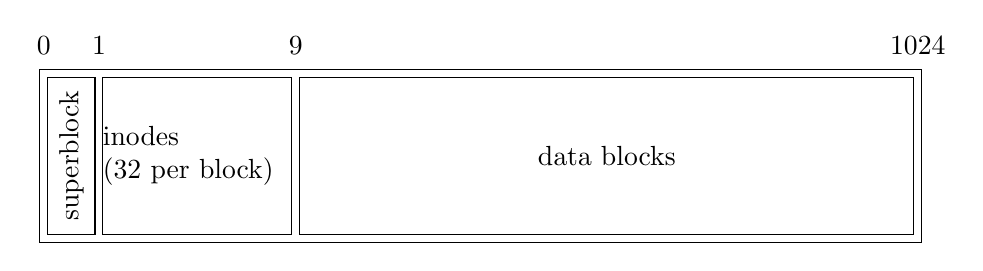
\begin{tikzpicture}
        % labels for disk block numbers and the bounding box
        \draw (-0.05,2.4) node {0};
        \draw (.65,2.4)   node {1};
        \draw (3.15,2.4)  node {9};
        \draw (11.05,2.4) node {1024};
        \draw (-.1,-.1)   rectangle (11.1,2.1);
        % the superblock box
        \draw (0,0)   rectangle (.6,2);
        \draw (.3,1)  node[rotate around={90:(0,0)}] {superblock};
        % the inodes box
        \draw (.7,0)  rectangle (3.1,2);
            % TODO centering text with align=center
        \draw (1.9,1) node[text width=2.4cm] {inodes\\(32 per block)};
        % the data blocks box
        \draw (3.2,0) rectangle (11,2);
        \draw (7.1,1) node {data blocks};
    \end{tikzpicture}
    \caption{The default disk layout for Weenix.}
\end{figure}

\subsection{Superblock}

The first block of the disk (block number zero) is called the superblock, which contains metadata about the file system. The important data fields inside it are the inode number of the root directory, the number of the first free inode, the first section of the free block list, the number of free blocks currently referenced in that section of the free block list, and the total number of inodes in use by the filesystem. The less important fields are the ``magic number'' for S5FS disks (used as a sanity check for the OS to determine that the disk you are reading is formatted as an S5FS disk), and the version number of S5FS we are using. The in-memory copy of the superblock is stored in a \texttt{s5\_super\_t} struct. For more information about the structure of the free block list, check out the section on \wlink{datablocks}{data blocks} below.

\subsection{Inodes}

Next, there is an array containing all the inodes for the file system. Each inode requires 128 bytes of space, and each disk block is 4096 bytes, so we store 32 inodes per block. Inodes are referred to by their index in the array, and are stored in memory as \texttt{s5\_inode\_t} structs.  Each inode is either free, or it corresponds to some file in the file system.

If an inode is not free, it represents a file presently on disk.  The inode holds of the size of the file, the type of the file (whether it is a directory, character device, block device, or a regular file), the number of links to the file from other locations in the file system, and where the data blocks of the file are stored on disk.

If an inode is free, it need only be marked as empty and contain the inode number of the next free inode in the free list (or \texttt{-1} if it is the last element in the list). This link is stored in the \texttt{s5\_freesize} field (you can think of that field as being a \texttt{union} whose interpretation depends on whether the inode is free or not).

The link count on an inode has a slightly different meaning based on whether or not Weenix is currently running. If Weenix is shut down, the link count simply reflects the number of directory entries which point to this file. However, while the OS is running, calling \texttt{vget()} on some file for the first time will result in a call to S5FS's implementation of \texttt{read\_vnode()}, which will increment the link count of the inode by one as long as the file is referenced by a vnode. Note that the link count will only be incremented when the file is first read from disk, not every time \texttt{vget()} is called on that file. Once the vnode's reference count drops to zero, the call to \texttt{vput()} will call S5FS's implementation of the \texttt{delete\_vnode()} function, which will decrement the link count of the inode. This extra link count is used to prevent the inode from being deleted from disk as long as some vnode still references it (even if the file has been unlinked from disk) so that any process that is using the file should have no problem reading it. As such, the link count for a new file should be two: one link from its parent directory and one from Weenix. Note that this is slightly different for directories; see the section on \wlink{directories}{directories} for details.

As mentioned above, the location of the data blocks for a file are also stored in the inode for the file. The inode itself keeps track of \texttt{S5\_NDIRECT\_BLOCKS} data block numbers directly, but this is not usually enough for a large-ish file. Luckily, S5FS inodes for ``large'' files also contain a pointer to an indirect block, which is a disk block filled with more data block numbers (in case it isn't clear: by ``pointer'' in this context we mean a disk block number, not a memory address). It is able to store up to \texttt{S5\_BLOCK\_SIZE / sizeof(int)} more block numbers. In a production file system, you should be able to support arbitrarily long files, which would require arbitrarily long indirect block chains (or, more likely, B-trees), but in Weenix we choose to only implement a single indirect block for simplicity. This means that there is a maximum file size; make sure you handle this error case correctly.

% picture of inode, indirect block, data blocks
\begin{figure}
    \centering
    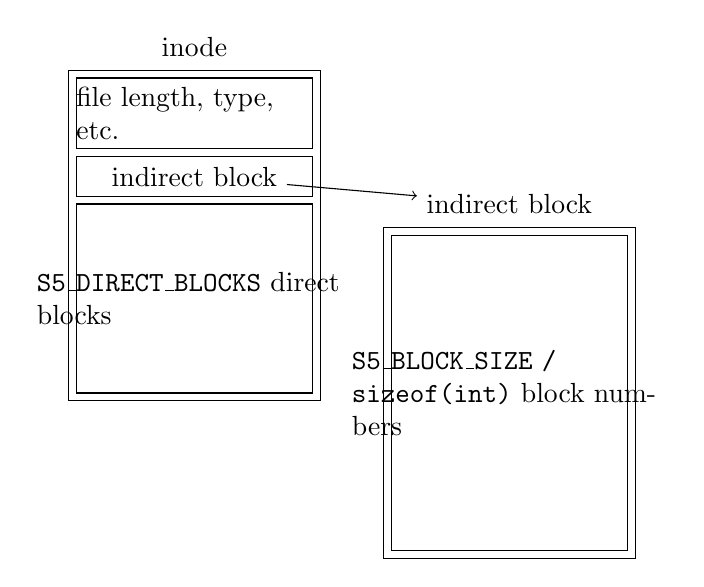
\begin{tikzpicture}
        % the inode label and bounding box
        \draw (1.5,4.4) node {inode};
        \draw (-.1,-.1) rectangle (3.1,4.1);
        % first data fields
        \draw (0,3.1) rectangle (3,4);
            % TODO centering text with align=center
        \draw (1.5,3.55) node[text width=3cm] {file length, type, etc.};
        % the indirect block label
        \draw (0,2.5) rectangle (3,3);
        \draw (1.5,2.75) node (indirect-pointer) {indirect block};
        % the direct blocks
        \draw (0,0) rectangle (3,2.4);
            % TODO centering text with align=center
        \draw (1.5,1.2) node[text width=4cm] {\texttt{S5\_DIRECT\_BLOCKS} direct blocks};
        
        % the indirect block
        \draw (3.9,-2.1) rectangle (7.1,2.1);
        \draw (5.5,2.4) node (indirect-block) {indirect block};
        \draw (4,-2) rectangle (7,2);
            % TODO centering text with align=center
        \draw (5.5,0) node[text width=4cm] {\texttt{S5\_BLOCK\_SIZE /\\sizeof(int)} block numbers};
        
        % arrow to indirect block
        \draw [->] (indirect-pointer) -- (indirect-block);
    \end{tikzpicture}
    \caption{An inode with an indirect block (data blocks not pictured).}
\end{figure}

While the default disk size gives you space for several hundred data blocks, the indirect block will allow a single file to use thousands of blocks. This might seem unnecessary, however it allows for the implementation of sparse files. If a file has a big chunk of zeros in it, Weenix will not waste actual space on the disk to represent them; it just sets the block index to zero. When reading a file, if a block number of zero is encountered, then that entire block should consist of zeroes. Remember that zero is guaranteed to be an invalid data block number because it is the block number of the superblock.

\subsection{Data Blocks} \label{datablocks}

Data blocks are where actual file contents are stored. They occur on disk after the inode array and fill the remainder of the disk. For simplicity, disk blocks and virtual memory pages are the same number of bytes in Weenix, although this is not necessarily true for other operating systems.

The contents of the data blocks are obviously dependent on what file they are filled with (except for directories, which also use data blocks but have a special format described below) unless they are in the free block list. Instead of a free list where each link only points to one more link, which would be wildly inefficient due to frequent seek delays, S5FS uses a list where each link in the list contains the numbers of many free blocks, the last of which points to the next link in the free list. The first segment of the free list is stored in the superblock, where up to \texttt{S5\_NBLKS\_PER\_FNODE} blocks are stored. The last element of this array is a pointer to a block containing \texttt{S5\_NBLKS\_PER\_FNODE} more free blocks, the last of which is a pointer to a block with more free pointers, and so on. The last free block in the list has a \texttt{-1} in the last position to indicate there are no more free blocks. After the second-to-last free block in the superblock's array is used, the next set of free blocks should be copied out of the next block, and then the block they were just copied from can be returned as the next free page.

% picture of free block list
\begin{figure}
    \centering
    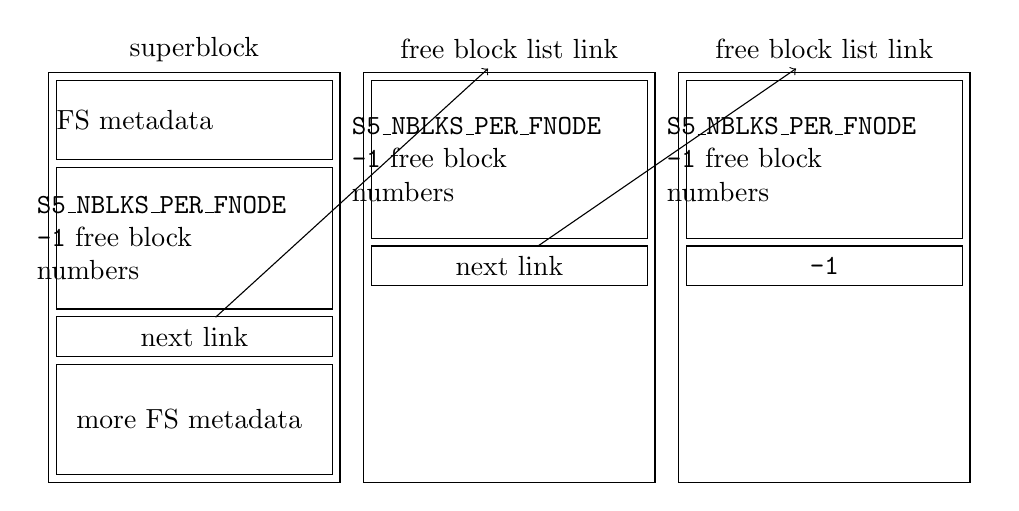
\begin{tikzpicture}
        % the inode label and bounding box
        \draw (1.75,5.4) node {superblock};
        \draw (-.1,-.1) rectangle (3.6,5.1);
        % first data fields
        \draw (0,4.0) rectangle (3.5,5);
            % TODO centering text with align=center
        \draw (1.75,4.5) node[text width=3.5cm] {FS metadata};
        % the direct blocks
        \draw (0,2.1) rectangle (3.5,3.9);
            % TODO centering text with align=center
        \draw (1.75,3) node[text width=4cm] {\texttt{S5\_NBLKS\_PER\_FNODE\\-1} free block\\numbers};
        % the next label
        \draw (0,1.5) rectangle (3.5,2);
        \draw (1.75,1.75) node (next-pointer) {next link};
        % other data fields
        \draw (0,0) rectangle (3.5,1.4);
            % TODO centering text with align=center
        \draw (1.75,.7) node[text width=3cm] {more FS metadata};
        
        % the next free block
        \draw (3.9,-.1) rectangle (7.6,5.1);
        \draw (5.75,5.4) node (next) {free block list link};
        \draw (4,3) rectangle (7.5,5);
            % TODO centering text with align=center
        \draw (5.75,4) node[text width=4cm] {\texttt{S5\_NBLKS\_PER\_FNODE\\-1} free block\\numbers};
        % the next label
        \draw (4,2.4) rectangle (7.5,2.9);
        \draw (5.75,2.65) node (next-next-pointer) {next link};
        
        % the next free block
        \draw (7.9,-.1) rectangle (11.6,5.1);
        \draw (9.75,5.4) node (next-next) {free block list link};
        \draw (8,3) rectangle (11.5,5);
            % TODO centering text with align=center
        \draw (9.75,4) node[text width=4cm] {\texttt{S5\_NBLKS\_PER\_FNODE\\-1} free block\\numbers};
        % the next label
        \draw (8,2.4) rectangle (11.5,2.9);
        \draw (9.75,2.65) node {\texttt{-1}};
        
        % arrow to next block
        \draw [->] (next-pointer) -- (next);
        
        % arrow to next-next block
        \draw [->] (next-next-pointer) -- (next-next);
    \end{tikzpicture}
    \caption{The free block list.}
\end{figure}

\subsection{Directories} \label{directories}

S5FS implements directories as normal files that have a special format for their data. The data stored in directory files is essentially just a big array of pairs of inode numbers and the filenames corresponding to those inode numbers. Filenames in S5FS are null-terminated strings of length less than or equal to \texttt{S5\_NAME\_LEN} (including the null character). Any entry with a zero-length name indicates an empty or deleted entry. Note that every directory contains one entry for ``\texttt{.}'' and one for ``\texttt{..}'', corresponding to the current directory and the parent directory, respectively, from the beginning of its existence to the moment it is deleted. The link count for a newly-created directory should be two (one reference from its parent directory, and one from the running copy of Weenix that just created it). The convention for weenix is that the self-reference from a directory to itself (\texttt{.}) is \emph{not} counted towards the link count.

\section{Caching}

At this point, you know a lot about how the on-disk filesystem looks and could probably inspect the disk block-by-block and understand what files are stored there. However, while working on this part of Weenix, you will not need to directly read and write from the disk, even in the most low-level functions. Instead, you will use the VM caching system to read blocks from disk into memory. You can then manipulate these pages in memory, and the pageout daemon will automatically handle writing them back to disk.

The Weenix caching system uses two different types of objects: page frames, which are each responsible for tracking one page/block of data, and memory objects, which are each associated with a number of page frames that hold the data for that memory object. In the codebase, the names for these objects are \texttt{pframe\_t}s and \texttt{mmobj\_t}s, respectively. Each memory object represents some data source, which could be a file, device, or virtual memory region. This means that page frames are used to reference the blocks of files, blocks of a device, and blocks of segments of memory. Specifically, page frames store some metadata about the page they hold and a reference to that page in memory. If a particular page of, say, a file hasn't been paged into memory, there will not yet be a page frame for that page.

To get a particular page frame from a memory object, you should call \texttt{pframe\_get()} on the memory object you wish to get the page from. The data stored in the page is stored at the location pointed to by the page frame's \texttt{pf\_addr} field. When a page frame has been modified, you should mark it as \wlink{pf-states}{dirty} so that it will be cleaned (the changes will be written back to disk) if necessary. The cleaning process uses callbacks in the disk's memory object to write the data back to disk.

To use an inode from disk, you must get its page from the disk memory object (the \texttt{S5\_INODE\_BLOCK()} macro will tell you which disk block to get) and then use the \texttt{S5\_INODE\_OFFSET()} macro to index into the page. When you are changing a file or the filesystem data structures, make sure that you remember to dirty the indirect block, inode, and superblock if necessary. Note the presence of the \texttt{s5\_dirty\_inode()} and \texttt{s5\_dirty\_super()} calls for this purpose. Remember that you should never clean pages yourself as either the pageout daemon or the Weenix shutdown sequence will take care of that automatically.

While working on S5FS, you may notice that there are two very similar methods for accessing the data on disk: calling \texttt{pframe\_get()} on the memory object for the block device (the disk) and on the memory object for the file. Therefore, it can sometimes be confusing which one to use. Although this may sound like common sense, it is important that you use a file's memory object every time you are dealing with a file, and use the block device's memory object when you are implementing pieces of the filesystem that are ``low-level enough'' to know how a file is split across multiple blocks on disk. If you accidentally use the disk memory object instead of the file memory object, you will be short-circuiting a couple layers of abstraction that will be necessary later on.

\subsection{Page Frame States} \label{pf-states}

As alluded to above, there are several states which a page frame can be in. At boot time, all page frames are \emph{free}, meaning they are waiting to be allocated. Some of the page frames will eventually be \emph{allocated}, at which point they are added to the allocated page frame list and filled with data. If a change is made inside their associated page of memory, they should be marked as \emph{dirty}.

The allocated page frame list is maintained to ease the implementation of the pageout daemon, which traverses the list and frees page frames and their associated memory pages. Note that any dirty pages will be cleaned (written out to disk) during this step, and non-dirty pages will simply be freed. The pageout daemon should only run when the system is out of memory, although you are allowed to call it other times as well if you choose. However, the use of the pageout daemon raises the question: how will you prevent a page frame from being freed while you are using it?

To solve this potential issue, page frames can also be \emph{pinned} while they are in use. Pages can be pinned multiple times; as long as the pin count of a page frame is greater than zero, it is guaranteed not to be cleaned or freed. This will also be important when you implement virtual memory, since page frames for some types of virtual memory regions will not be backed by disk and can therefore never be safely cleaned or freed. When a page is pinned, it is removed from the allocated frame list and added to the pinned list, and the reverse happens when the last pin is removed.

The only time during S5FS where you should pin pages is when it is possible that your code will block after finding a page frame and before using that frame, since those are the conditions under which the pageout daemon could free the page, causing a memory corruption bug that will be difficult to reproduce. If you are unsure whether some code path might block, it is safer to pin any page frames you are using than not to do so. When you are done using the page frames, make sure you unpin them so that you do not run out of memory.

Finally, to protect page frames from making ill-formed state transitions, page frames can be marked as \emph{busy} while they are in the middle of a state transition. Any concurrent attempts to modify a page frame (not necessarily the page it points to) should block until it is no longer busy.

\subsection{Lazy Cleaning}

One noteworthy feature of Weenix's caching system is that it does not uncache any pages of a file until either the system is out of memory (the pageout daemon may write back some or all of the changes at this point) or Weenix shuts down (the page frame system writes back its changes). This feature was added to improve cache performance for files that are closed and reopened frequently.

Each time \texttt{vput()} is called on a file, the S5FS implementation of \texttt{query\_vnode()} is run to check if the file is still referenced by some directory on disk or some vnode in memory. If it has been deleted from every directory it was present in and you are \texttt{vput()}ing the final memory reference to the file, the blocks of that file that are cached in memory can simply be freed (even if they are dirty) since nobody will ever need to use them again. Otherwise, they are left to be cleaned up at some later point. If you notice that your filesystem is working but none of your changes are being propagated to disk, you may want to check to see if this code path is running.

\section{Error Handling}

You always need to check for things that can go wrong. When an error condition occurs, you should return \texttt{-errno} where \texttt{errno} is the error number that indicates the type of error that occurred. For example, if you run out of free data blocks when attempting to write to a new block of a file, you should return \texttt{-ENOSPC}. You should \emph{always} check the return value from non-void functions you call, and if the returned value is negative you often need to propagate it up. Returning \texttt{-1} is not correct.

However, it is also important that your VFS code check for as many errors as possible, so that each file system that it runs need not check the same error cases. If you know that some error condition should always be dealt with at the VFS layer, you should assert that it does not occur in the S5FS layer to identify bugs in your implementation while you develop.

We have tried to indicate some errors that you should check for in the comments, but we have probably not mentioned all of them, so you should go over your code thoroughly to make sure that you handle all possible errors.

\section{Getting Started}

You need to implement:

\begin{itemize}

\item The high-level system calls for S5FS (the VFS interface).  Many of these will have a name such as \texttt{s5fs\_[name]} with a corresponding VFS call named \texttt{do\_[name]}.

\item The low-level subroutines.  These subroutines represent common functionality that may be useful to reuse in many of the high-evel system calls.

\item A few memory management routines (such as \texttt{pframe\_get()}).  This is to understand a little better how the caching system works.

\end{itemize}

\section{Testing}

Your test cases should demonstrate clearly that all functions have been tested properly. While much of the functionality of S5FS will be tested by the tests you used for VFS, there are several cases that may require a bit more thought:

\begin{itemize}
    \item Indirect blocks. (The \texttt{hamlet} file on your virtual disk is provided as an example of a file which needs an indirect block, but don't forget to check the case where you need to allocate one at runtime as well.)
    \item Sparse blocks.
    \item Running out of inodes, data blocks, or file length.
    \item Shutting down and rebooting does not erase your changes.
\end{itemize}

Be sure that your link counts are correct (\texttt{calculate\_refcounts()} will calculate the counts for you). Note that you \emph{must} make sure you are actually shutting down cleanly (i.e. see the ``Weenix halted'' message). Reference count issues will prevent Weenix from shutting down cleanly.

To ease the difficulty of debugging your file system code, we have provided a couple of utilities to help you develop. The \texttt{fsmaker} utility will come in handy for inspecting blocks, inodes, and other data structures on your virtual machine's disk. To read more about how to use \texttt{fsmaker}, run \texttt{fsmaker --help} from the root of your development directory. Your disks are stored in files on the host operating system (the \texttt{user/disk*.img} files), and must be passed to \texttt{fsmaker} as an argument. Also, running the \texttt{./weenix} script with the \texttt{-n} option will create a brand new disk for you and fill it with a bunch of sample files and directories. To begin this assignment, you must use this option at least once, otherwise you will not have a disk to work with.

        \chapter{Virtual Memory}
\label{vm}

\section{Introduction}

At this point, your Weenix contains a threading library, some thin wrappers around device drivers, and basic file system support with a caching layer. By the end of this assignment, Weenix will be a full operating system. With the addition of virtual memory, your kernel will start managing user address spaces, running user-level code, and servicing system calls. After completing this project, everything you did before will seem insignificant.

This assignment is substantial, and also very prone to difficult bugs. Before you begin, make sure the rest of your kernel is functioning exactly as you expect. You will undoubtedly uncover bugs in old code throughout the course of this assignment, but minimizing the number you find before you start will be helpful. Make sure to start early and ask questions frequently; it is very easy to get lost in this assignment.

Remember to turn the \texttt{VM} project on in \texttt{Config.mk} and \texttt{make clean} your project before you try to run your changes.
% TODO improve next paragraph

Because VM bugs can spring up in code you wrote months ago, this is where you will probably find out whether or not your implementations of the previous assignments are up to par. We would like to point out that there are several Weenix- and OS-specific debugging tools and techniques in Appendix \ref{Debugging} which will be \textit{extremely} useful if you have not been using them so far.

\section{Virtual Memory Maps}

The first thing you should do in this assignment is write the code for managing a process' virtual address space. The virtual address space for a process (also known as its ``memory map'') is stored as a linked list of virtual memory areas (also referred to as ``memory regions''), each of which correspond to some memory object which provides pages of memory to the process on demand. As you have likely already realized, this means that everything from files to disks can be mapped into the address space of Weenix processes, and it should now make even more sense why we used memory objects extensively in the last assignment instead of reading and writing directly to disk. Of course, some memory areas will not correspond to existing data (the stack and heap, for instance). We will explain how that works in the section on \wlink{anon}{anonymous objects}.

In order to manage address spaces, you must maintain each process' list of virtual memory areas. Each memory region is essentially a range of virtual page numbers, a memory object, and the page offset into that memory object that the first page of the virtual memory area corresponds to. Make sure that you understand why these numbers are all stored at page resolution instead of byte (address) resolution. You must keep the areas sorted by the start of their virtual page ranges and ensure that no two ranges overlap with each other. There will be several edge cases (which are better documented in the code) where you will have to unmap a section of a virtual memory area, which could require splitting an area or truncating the beginning or end of an area.

While there is very little conceptually difficult code to write in this section of the assignment, off-by-one bugs are extremely common and become very difficult to track down later on, so unit-testing this code is a good idea.

\section{Page Fault Handler}

After your memory maps are working, you will need a way to actually load the data into memory when a process attempts to access it. This is done by the page fault handler. The page fault handler is triggered by a processor interrupt when a process attempts to access an address for which it has no lookup entry in the page table or the permissions on that entry do not allow the type of access that is being attempted.

At this point in the project, any page faults that have occurred have resulted in a kernel panic. That is because Weenix does not support kernel-level page faults, meaning that the entire kernel address space must reside in memory at all times. This functionality is written into a wrapper for the page fault handler you will write which short-circuits kernel page faults. More details on how this function works can most easily be found in the code.

The combination of the page fault handler and the virtual memory maps should be enough to get a very simple page fault to occur in a userland program. At this point, you can set up a userland program to run from inside the \texttt{init} process by running \texttt{kernel\_execve()}, passing the path to any program on your (virtual) disk as an argument. Similar to the \texttt{exec()} system call, this will replace the memory map of the current process to set up another program to run, but it will be better than \texttt{exec()} in this case because the setup is done exclusively in kernel space, so it can be used before you have a fully functional userspace. When the program begins, it should cause a page fault to be generated. This is your first step towards having a functional userland.

A simple implementation of the page fault handler will be enough to start with, but eventually this will be a relatively logic-heavy function. First, the page fault handler should search for the virtual memory area containing the address that was faulted on. Then, the permissions of this area should be checked against the flags variable that is passed to the handler, which tells the handler whether the attempted access is a read or a write. If the memory area containing the accessed page is not found or the permissions would make this access illegal, the current process is killed with an exit status of \texttt{EFAULT}. Of course, if Weenix supported UNIX signals, it would send a \texttt{SIGSEGV} signal instead.

Once the virtual memory area is found, Weenix must search for the missing page and map it into the page table of the current process so that the access can be retried using the virtual address of the page that's being added and the physical address where it resides. Fetching the missing page will require a lot of help from the page frame caching system, namely for looking up the page and dirtying it if the access is a write. This, in turn, will rely on two new types of memory objects you will need to implement.

\subsection{The Memory Management Unit}

In order to map the virtual address to its corresponding page of memory, you will need to use the page table functions. A good portion of memory management is done for you, but you will have to fill in page table entries when page faults occur, flush the translation lookaside buffer (TLB) when necessary, and manage copy-on-write pages yourself. You will also need to make sure that pages which are not backed by files remain pinned, so they do not get paged out by accident.

\section{Memory Management}

As you have implemented it currently, the caching layer of Weenix works exclusively for pages of files or disks that have been mapped into memory. You will extend it by creating memory objects which will provide two new types of memory which are not backed by any on-disk structures.

\subsection{Anonymous Objects} \label{anon}

So far, you have used the memory objects of your block device and files to fill page frames as you needed data from disk, but it does not make sense to back some virtual memory areas, such as a process' stack, with data on disk. What you often want is objects which initialize pages by filling them with zeroes and pin their pages in memory as long as the process is using them. These are known as anonymous objects since they are not backed by any persistent data (which would have a filename associated with it). Anonymous objects are relatively simple to implement, so look for a better description of how they work in the code comments.

Notably, anonymous objects cannot be paged out in Weenix. The designers chose not to implement this feature because memory pressure will rarely be an issue in your operating system, and implementing a swap space is not terribly interesting or vital to implement as a result.

\subsection{Shadow Objects}

Anonymous objects are easy to implement, however you will also need a much more sophisticated form of memory object called a shadow object to implement \texttt{fork()}. These will be used to implement copy-on-write for privately-mapped blocks that are accessed after forking. Because of how involved shadow objects must be, you should refer to lecture slides or the book for more general information about how and why they are used. The rest of this section will only cover how to implement them in Weenix.

To implement shadow objects, it will be extremely helpful to understand how the methods of memory objects are called during a page lookup or dirty operation. If you don't remember this well from the last assignment, we recommend that you go back and either re-read the relevant sections of the last assignment or search through the code paths in question and draw a graph showing what functions in the page frame system call what functions in the related memory objects.

The main difference between shadow objects and other types of memory management objects is that shadow objects can be part of arbitrarily long chains of memory objects. Therefore, many calls to shadow objects will be rerouted to the object that is being shadowed, or occasionally to the root object in a tree of memory objects, which cannot be a shadow object. At a high level, this is similar to how file memory objects forward requests to the disk memory object, but in practice it ends up seeming a lot more recursive when implementing shadow objects since there is no translation layer as there was between file block numbers and disk block numbers. However, shadow objects are still responsible for storing some data and, more importantly, causing copy-on-write to work after a \texttt{fork()} has taken place.

One potential problem with shadow objects is that the chains must be cleaned up when the process that creates them exits to avoid temporary memory leaks. Ideally, this could happen at process exit. A process exiting might cause a shadow object's refcount to drop to one, at which point the pages attached to the object could be reassigned to the single shadow object beneath it, and the object itself could be deallocated. However, this would require the shadow object to know what its remaining child is and, at the moment, shadow objects do not maintain a list of their children.

This apparent design flaw leaves two other avenues for shadow chain cleanup. First, there is a shadow daemon known as \texttt{shadowd} which was built for this purpose. It should be invoked when the kernel is out of memory (this code is already written) or when a shadow object which can be cleaned up is created (you can tell this by checking for it when you remove either of its child shadow objects). To enable the shadow daemon, just set \texttt{SHADOWD=1} in the project environment settings. The shadowd code exists as a testing tool, but you should \emph{not} use it for your final product. 

The second method would be to collapse shadow chains during \texttt{fork()}. This requires a relatively easy traversal of the forking process' object chains, where you shift the pages from any objects with a single child down to their child and then deallocate the objects. You should implement this for your final product inside your fork logic. 

\section{System Calls}

System calls are the only way user processes can communicate with the Weenix kernel directly. The way that system calls are generated from user space is by generating a software interrupt (using the x86 \texttt{int} instruction) with the arguments to the system call stored in the registers or on the stack. This causes an interrupt in the kernel, where the number in an agreed-upon register designates which system call is being used, and then the corresponding system call function is actually called to handle the request after the arguments have been parsed out of their registers. Most of the system calls have already been written for you, however, in order to give you some understanding of the process involved, you will need to write a few yourself.

\subsection{Kernel System Call Interface}

You will need to implement the kernel targets for \texttt{read()}, \texttt{write()}, and \texttt{getdents()}. While most of what you need to do should be pretty self-explanatory after reading through other system call implementations, you must also write two helper functions to check accesses to user memory from within the kernel.

\subsection{Accessing User Memory}

The code to handle traps and access user memory from the kernel has been written for you. However, many of these functions need to check to see if a region of user memory is a valid section of the process' address space. To check this, you will need to implement \texttt{addr\_perm()} and \texttt{range\_perm()}, which will rely on your virtual memory map code.

\subsection{Running Userland Programs}

Once you have implemented the page fault handler, anonymous objects, and \texttt{write()}, you should be able to run a variety of simple user-level programs. Of course, the first you should try to get running should also be one of the simplest, so we recommend \texttt{hello}, which should print ``Hello, world!'' to the screen. To run correctly, this will require a mostly-functional page fault handler to fill in pages as the process attempts to access them; otherwise, the operating system will probably go into an infinite loop, trying to access the same address over and over using the page fault handler, but never adding the correct entry to the page table. Some other simple programs that you should be able to run are \texttt{args} and \texttt{uname}.

If you are having trouble getting \texttt{hello} to run and suspect that your anonymous object or \texttt{write()} implementations might be at fault, you should try the \texttt{segfault} program instead and ensure that it exits with a status of \texttt{EFAULT}. If it doesn't (if, for instance, you run into the infinite loop problem described above), this means the bug is probably in your page fault handler.

After getting \texttt{hello} or \texttt{segfault} running, congratulations! You've just gotten your first userland program working! Celebration techniques are myriad, but we recommend dancing around a bit, and maybe taking a shower.

At this point, it will be useful to look at the \wlink{Debugging}{debugging} appendix covering how to inspect the progress of a user-level process using a debugger. Although you may not need it yet, we assume that you will want it very soon.

\subsection{VM-Related System Calls}

After you get some initial test programs running, you can start to think about implementing a variety of VM-related system calls. For the functions in this section, we recommend that you check out the documentation in the \texttt{man} pages for more information.

\texttt{mmap()} and \texttt{munmap()} are the most simple and obvious of the functions in this category. They allow user processes to map files into memory, create private or shared memory regions, and remove areas of their address space. The majority of these functions will end up being error-checking, since you wrote the main logic for them in the virtual memory map code.  Note that the Weenix memtests expect you to use the \texttt{VMMAP\_DIR\_HILO} flag.

\texttt{brk()} is similar in conceptual difficulty. Calling \texttt{brk()} changes the length of the memory region acting as the heap, but the pointer passed as an argument to \texttt{brk()} is not required to lie on a page boundary, and the beginning of the heap sometimes starts halfway through the last page of another memory region. This means that the edge cases for \texttt{brk()} can be a bit annoying, but there's nothing conceptually difficult to grasp here. There are some robust user-level tests for much of this functionality, so rather than spending a lot of time getting it right before testing, we recommend starting with something naive and gradually fixing it to pass the tests after you can run them in userland.

\section{\texttt{fork()}}

Although it is also a VM-related system call, \texttt{fork()} is an entirely different animal from \texttt{mmap()} and friends. A good implementation of the previous sections is essential; \texttt{fork()} is complicated enough without having to debug the rest of your VM code at the same time. The \texttt{man} pages, while useful as always, will not be as helpful for \texttt{fork()} as for the other system calls, so most of the documentation for \texttt{fork()} is given here.

\texttt{fork()} is a moderately complicated system call. We present it here as one long algorithm, but it will make your life much easier if you break it down into separate subroutines. Close attention to detail will help you; an under-debugged \texttt{fork()} can cause subtle instabilities and bugs later on.

Bugs in the virtual memory portion of \texttt{fork()} tend to cause bizarre behavior: user process memory may not be what it ought to be, so almost anything can happen. The user process may end up executing what should be data, jumping into the middle of a random subroutine, etc. These sorts of bugs are \emph{very} difficult to track down. For this reason, you should code more defensively than you may be used to. Assert everything you can, \texttt{panic()} at the first sign of trouble, and include apparently unnecessary sanity checks.

Above all, be sure you really understand the algorithm before you start coding. If you try to implement it before you understand what you are trying to do, you will write buggy code. In all likelihood you will then forget that you have written buggy code, and waste time debugging code that you should have thrown away. We know this because it has happened to us.

Note that these steps are not all in the correct order; consider the order in which you do them, keeping in mind what kind of cleanup you will need to do if one of them fails. Look out for steps which cannot be undone.

\begin{itemize}
    \item Create a new process using \texttt{proc\_create()}.
    \item Copy the \texttt{vmmap\_t} from the parent process into the child using \texttt{vmmap\_clone()} (which you should write if you haven't already). Remember to increase the reference counts on the underlying memory objects.
    \item For each private mapping in the original process, point the virtual memory areas of the new and old processes to two new shadow objects, which in turn should point to the original underlying memory object. This is how you know that pages corresponding to this mapping are copy-on-write. Be careful with reference counts. Also note that for shared mappings, there is no need to make a shadow object.
    \item Unmap the userland page table entries and flush the TLB using \texttt{pt\_unmap\_range()} and \texttt{tlb\_flush\_all()}. This is necessary because the parent process might still have some entries marked as ``writable'', but since we are implementing copy-on-write we would like access to these pages to cause a trap to our page fault handler so it can dirty the page, which will invoke the copy-on-write actions.
    \item Set up the new process thread context. You will need to set the following:
        \begin{itemize}
            \item \texttt{c\_pdptr} - the page table pointer
            \item \texttt{c\_eip} - function pointer for \texttt{userland\_entry()}
            \item \texttt{c\_esp} - the value returned by \texttt{fork\_setup\_stack()}
            \item \texttt{c\_kstack} - the top of the new thread's kernel stack
            \item \texttt{c\_kstacksz} - size of the new thread's kernel stack
        \end{itemize}
    \item Copy the file table of the parent into the child. Remember to use \texttt{fref()} here.
    \item Set the child's working directory to point to the parent's working directory. Once again, don't forget reference counts.
    \item Use \texttt{kthread\_clone()} (which you should write if you haven't yet) to copy the thread from the parent process into the child process.
    \item Set any other fields in the new process which need to be set.
    \item Make the new thread runnable, which will add it to the run queue.
\end{itemize}

Remember that the only difference between the parent and child processes is the return value of \texttt{fork()}. By 32-bit x86 convention, this value is returned in the \texttt{eax} register, which should be set in the context values of both threads. You should also revisit your implementation of the \texttt{proc\_exit()} function to make sure that your implementation is releasing all resources it should.

Note that a simpler, less correct implementation of \texttt{fork()} can function without actually using shadow objects, as long as you don't care what happens to whichever process (parent or child) wakes up last from the syscall. If you're having trouble getting shadow objects to work correctly, you can write \texttt{fork()} without them for testing purposes.

\section{Odds and Ends}

Finally, there are a number of other functions which you might remember seeing in earlier assignments spread throughout the kernel which you need to find and either write or update. These functions are all fairly small, but if you miss one, some things will break. Two examples are \texttt{special\_file\_mmap()} and \texttt{proc\_kill\_all()}. Once you get the last of these finished, you should be able to test your kernel with any binary file you find on the Weenix file system.

\section{Testing}

Testing your code at this point becomes rather difficult, since you must be able to create data and text in user land and execute it. This is an order of magnitude more difficult than creating kernel-mode threads as you have in past assignments. Thankfully most of the gory details have been taken care of for you (take a look at \texttt{kernel/api/elf32.c} and \texttt{user/ld-weenix/} if you are a masochist).

\subsection{Userland Tests}

Once you have functioning userland execution and a working \texttt{fork()} function, you are ready to complete your Weenix system by running the userland binaries we provide for you. All you need to do is call \texttt{kernel\_execve()} in your init process. You should execute the binary \texttt{/sbin/init}, which should start 3 shells (one in each terminal window). These shells will allow you to execute any of the provided binaries (roughly in order of difficulty):
\begin{itemize}
    \item \texttt{/usr/bin/segfault} - Even simpler than hello, this should just segfault on address \texttt{0x0}. Good if you're having a lot of trouble getting hello to run.
    \item \texttt{/usr/bin/hello} - A simple ``Hello world!'' test. Getting this to execute properly should be a big step in VM.
    \item \texttt{/usr/bin/args} - Prints command arguments.
    \item \texttt{/usr/bin/fork-and-wait} - Simple program which forks, and prints out everything of note.
    \item \texttt{/bin/uname} - Prints system information.
    \item \texttt{/bin/stat} - Prints information about a file.
    \item \texttt{/usr/bin/kshell} - Traps into the kernel and starts a kshell.
    \item \texttt{/bin/ls} - List the contents of a directory.
    \item \texttt{/sbin/halt} - Kills all processes and shuts the system down.
    \item \texttt{/usr/bin/wc} - Counts characters, words and lines.
    \item \texttt{/bin/sh} - The shell itself. Yay subshell fun!
    \item \texttt{/usr/bin/spin} - Executes ``\texttt{while(1);}''.
    \item \texttt{/usr/bin/forkbomb} - A forkbomb test which should theoretically run forever.
    \item \texttt{/usr/bin/stress} - A test to stress various parts of your system and then run a forkbomb.
    \item \texttt{check} - Contains checks for various test cases (this is a shell built-in command).
    \item \texttt{/usr/bin/vfstest} - Lots of VFS tests (error conditions, etc.).
    \item \texttt{/usr/bin/memtest} - Lots of memory management tests (mmap and brk).
    \item \texttt{/usr/bin/eatinodes} - Devours filesystem resources.
    \item \texttt{/usr/bin/eatmem} - Devours kernel memory.
    \item \texttt{/bin/ed} - \texttt{ed} is the standard text editor.
\end{itemize}

The shell also has a bunch of builtins. Type \texttt{help} in a shell to see a list of them. In particular, \texttt{repeat} and \texttt{parallel} can be very useful for stress testing your kernel.

\subsection{A Relatively Difficult Test Suite}

In addition to just having commands which work individually, you should be able to stress the hell out of your system. Run lots of difficult commands (\texttt{forkbomb}, \texttt{eatmem}, etc.) simultaneously, use different terminals at once, \texttt{halt} in the middle of all this, and so on. This type of testing can frequently be quite random, so here is a more systematic list of some things you can try. Make sure you start with a fresh disk.

\begin{itemize}
    \item \texttt{cat hamlet}
    \item \texttt{cat hamlet > hamlet2}
    \item \texttt{halt} (to shut down, then make sure the changes still exist on disk when you reboot)
    \item \texttt{rm hamlet}
    \item \texttt{cat /dev/null > foo}
    \item \texttt{ln foo bar}
    \item \texttt{cat README > foo}
    \item \texttt{cat bar}
    \item \texttt{check all} (do this three or four times in a row)
    \item \texttt{vfstest}
    \item \texttt{memtest} (do this three or four times in a row)
    \item \texttt{parallel vfstest -- vfstest}
    \item \texttt{parallel memtest -- memtest}
    \item \texttt{vfstest} and then \texttt{halt} while running (use \texttt{repeat} to re-run \texttt{vfstest} if it finishes too quickly)
    \item \texttt{memtest} and then \texttt{halt} while running
    \item \texttt{forkbomb} and then \texttt{halt} while running
    \item \texttt{forkbomb} and then \texttt{eatmem}
\end{itemize}

An easy way to make these tests harder is to check the kernel memory allocators for any leaks. See the \wlink{Debugging}{debugging} appendix to see how to do this. You may also want to test what happens when Weenix runs out of disk data blocks. To do this, set the \texttt{DISK\_BLOCKS} variable to 2048 if it is not already, and then re-run Weenix with a fresh disk and execute the commands below.

\begin{itemize}
    \item \texttt{cat hamlet >> hamlet} (this should reach the maximum file size and then exit)
    \item \texttt{vfstest} (this should work - the disk is not yet filled)
    \item \texttt{cat README >> README} (this should fill the disk but not quite reach the maximum file size)
    \item \texttt{vfstest} (this should fail to run most of the tests due to no disk data blocks being available)
\end{itemize}

\subsection{Dynamic Linking}

Once you feel everything is in good shape, enable the \texttt{DYNAMIC} variable and recompile the project from scratch. This will cause your userland libraries to be dynamically linked, which puts much more stress on your VM (especially \texttt{mmap()} code). This essentially adds another layer of indirection between the executable being run and the library calls it's attempting to run, where \texttt{ld-weenix} can link the library calls that are used into the original binary at runtime. Unfortunately, this also makes it even more difficult to debug what the user process is doing; if you are interested in setting breakpoints in the user process with dynamic linking, check out the \wlink{Debugging}{debugging} appendix for more information.

Turning dynamic linking on will make the above tests even more thorough. For instance, the test using \texttt{forkbomb} and \texttt{eatmem} simultaneously is notoriously hard to get right in the presence of dynamic linking - a phantom bug might cause your \texttt{pageoutd} to thrash back and forth between two pages if you're not careful.

\section{Conclusion}

We hope you've enjoyed working on Weenix and that you learned a lot. Good luck finishing your project, and don't forget to read the \wlink{Debugging}{debugging} appendix if you run into problems or need more ideas about where to look!

    \part{Appendices}
        \appendix
        \chapter{Extra Assignments}
\label{extra-asgn}

% TODO this chapter needs to be cleaned up and organized a bit better, and parts are a bit too sarcastic for general publication

The features listed on this page are not extra credit. \textbf{There is no extra credit in Weenix.} Your grade is based on how well you complete the core Weenix requirements. Therefore trying to implement these things can only hurt your grade and distract you from what is really important in life. The only thing to be gained by foolishly ignoring this warning is a deeper understanding of Weenix and bragging rights. \textbf{We will look unfavorably on someone who has implemented some of these, but has problems with the core Weenix projects.}

Some items on this page include descriptions on when it is feasible to implement them, be aware however that you should always keep around a copy of your work which does not contain your work on extra features in case you break something. \textbf{Having a broken Weenix because you tried to implement one of these features is not acceptable.} This is particularly important to remember because you might implement a feature between \wlink{vfs}{VFS} and \wlink{s5fs}{S5FS} only to find later when working on \wlink{vm}{VM} that you broke something badly.

Also note that the course staff will only be able to provide limited help with these features. Some of the features have been implemented in the staff version of the code, others have been attempted and abandoned, still others are random whims which may or may not be impossible.

\section{Realistic projects}
If you ignored the warning above then this is the place to start. These are features which are known to be possible because someone has either done so or it has been planned. This means you will get some description here on how to implement it and there might even be helpful code already in Weenix.

\subsection{Multithreaded processes}
This task has a bunch of places in code that are marked by the \texttt{\_\_MTP\_\_} symbol (which must be enabled by setting ``\texttt{MTP = 1}'' in \texttt{Config.mk}), and the kernel is designed around it anyway. This is a relatively straightforward addition to the kernel.

\subsection{Current working directory}
This will add a system call which looks up the full path name of the current working directory of the current process and is marked in the codebase with the symbol \texttt{\_\_GETCWD\_\_}, which can be enabled by setting ``\texttt{GETCWD = 1}'' in \texttt{Config.mk}. This should not be too difficult at all.

\subsection{File system mounting}
One important missing feature in our VFS implementation is mount points. We have a root file system (\texttt{ramfs} if you are working on \wlink{vfs}{VFS}, \texttt{s5fs} if you are working on \wlink{s5fs}{S5FS}), but normal UNIX allows you to access multiple file systems by ``mounting'' additional file systems on directories in your virtual file system layer.

For more information on mount points we refer you to the \texttt{mount(2)} man pages, the \texttt{umount(2)} man pages, the lecture slides, and the text book.

Before you begin, there is already a significant amount of code in Weenix for this feature; however, by default it is not compiled. To compile this code change the line ``\texttt{MOUNTING = 0}'' in \texttt{Config.mk} to ``\texttt{MOUNTING = 1}''. Also, remember to run:
\begin{verbatim}
$ make clean\end{verbatim}

% TODO cscope
You should use \texttt{cscope} to search for all instances of the C symbol \texttt{\_\_MOUNTING\_\_} in Weenix to see exactly what has changed to allow mounting to happen. Notice that \texttt{struct fs} in \texttt{fs/vfs.h} now has a new field called \texttt{vn\_mount}.

The biggest change caused by changing the \texttt{MOUNTING} flag is the behavior of \texttt{vget()} (even though very little code changed, the behavior is completely different). The easiest way to think of the behavior of the new \texttt{vget()} is like this:
\begin{verbatim}
vnode_t* new_vget(args) {
    vnote_t* vn = old_vget(args);
    if (!error) {
        return vn->vn_mount;
    } else {
        return error;
    }
}\end{verbatim}

The purpose of this change is to make the integration of mounting as seamless as possible. Normally \texttt{vn->vn\_mount == vn} and therefore most of the time this new behavior is identical to the old one; however, simply by setting the \texttt{vn\_mount} field the \texttt{vget()} function automatically traverses into mounted file systems for us. The only cases we need to worry about are when we are leaving a mounted file system (e.g. following a \texttt{..} path from the root of a mounted file system).

The easier part of implementing mounting is filling in some functions which have been left blank (but fully commented!) for you. In \texttt{fs/vfs.c} this is:
\begin{verbatim}
int vfs_mount(struct vnode *mtpt, fs_t *fs);
int vfs_umount(fs_t *fs);\end{verbatim}
in \texttt{fs/vfs\_syscall.c} there is also:
\begin{verbatim}
int do_mount(const char *source, const char *target,
             const char *type);
int do_umount(const char *target);\end{verbatim}

You will also want to read the Hackers Guide section about reference counting for information about special conventions used when reference counting mount point \texttt{vnode\_t}s.

Now comes the hard part: implementing these functions is not enough. As was noted in the previous section, setting up the \texttt{vn\_mount} field will allow us to enter mounted file systems. However following \texttt{..} paths out of mounted file systems still needs to be special cased. You will need to think about the code you wrote for \wlink{vfs}{VFS} and which code will need to be different in order to handle mounting correctly. The amount of code you will need to write is small, but you need to find the right functions to write it. All of the code should go into functions which you wrote for \wlink{vfs}{VFS}. You do not need to modify functions which you wrote for other projects or functions which you did not write originally. Also remember some of the system calls have errors specific to mounting which you might not have worried about before (e.g. What happens when you try to link a file from one file system onto another? Why is this an error?).

\subsection{Userspace preemption}
Definitely possible. The basic idea is that a timer interrupt is scheduled to occur every several milliseconds. The interrupt context then looks at the thread which was interrupted. If the thread was in userspace it is safe to just put that thread on the run queue and switch into the context of another thread (thus preempting the userland process). If the interrupted thread was in the kernel, we do not want to arbitrarily preempt it (preemptible kernels lead to kernel hacker hell). Instead, we set a flag on the thread to mark it as preempted and allow it to continue. When a thread returns from kernel land into user land the flag should get checked and if it is set the preemption should happen at that point. Make sure you understand all of this before you start or things will get messy.

So, do you gain anything from doing this? Actually, the effects are very visible and very satisfying. You will be able to run \texttt{vfstest} and \texttt{cat hamlet} at the same time and they will all look like they are running at the same time (assuming you set a good preemption time) while your fellow students will have very visible times when one operation stops working while the other is running. Also, your Weenix will not hang while you \texttt{cat /dev/zero} to \texttt{/dev/null}.

To get started on this enable the compile time flag and check out the code in \texttt{kernel/util/time.c}.  It sets up the timer interrupts but you have to fill in what to do once they happen.

\subsection{Pipes and synchronous multiplexing}
One thing that greatly increases the power of shells and other programs is pipes, because they all for simple inter-process communication. This is not difficult to add to the standard Weenix, and some support code has been included to help you. Enable the pipe subsystem by setting \texttt{PIPES = 1} in \texttt{Config.mk} and look in \texttt{fs/pipe.c} to get started. Make sure you understand how the \texttt{pipe(2)} system call works. It has the following signature:

\begin{verbatim}
int do_pipe(int pipefd[2]);\end{verbatim}
If successful, this call will fill the supplied \texttt{pipefd} array with a file descriptor representing the end of the pipe for reading, and then a file descriptor representing the end of the pipe used for writing.

Once you are done with that, you have a use case for synchronous I/O multiplexing, which is where a program can wait for any of multiple file descriptors to become ready. This is typically implemented using the \texttt{select(2)} and \texttt{poll(2)} system calls. Look those up for more information, but the basic premise is that you want to check if any of the file descriptors the user put in are ready for whatever operation they requested, and if they are not, have some way to sleep until one or more of them is ready.

These syscalls are filesystem-oriented and rely on some extensions to \texttt{vnode} operations that you won't have to touch for normal Weenix. For example, because pipes have to know when all of the readers of a pipe have closed their file descriptors, the pipe must keep an accurate count of how many files have it open for reading and writing. This requires new \texttt{vnode} operations that also take the \texttt{file} which is getting a reference (called \texttt{acquire}) or putting a reference (called \texttt{release}) to the \texttt{vnode}. Requesting events from \texttt{vnode}s for multiplexing will require an operation typically called \texttt{poll}, which checks whether reading or writing will block, among other things.

\subsection{Asynchronous disk driver}
It would be cool to support an asynchronous disk driver. To do this would require a decent amount of restructuring in the driver code, but is doable given a bit of time and effort. After this is done, you could potentially add asynchronous user I/O support as well (although this is a harder problem because in most Unix distributions the notification of a completion is done through signals).

\subsection{Better scheduling}
After you have finished implementing processes and threads, you should know the basics, but it might be a bad idea to try making too many big changes to Weenix before you have really gotten exposed to everything. % TODO processes and threads

The current Weenix scheduler is rather primitive as it has no sense of priorities and makes no attempt to do any ``clever'' scheduling; it is purely first come first serve. Here are some helpful suggestions:
\begin{itemize}
    \item Professor Doeppner's lecture (only available to Brown students) on scheduling contains plenty of information on different scheduling algorithms (you might also check the textbook).
    \item The CS167 students implement a slightly more advanced scheduler for their threading library assignment. You might be able to get some inspiration from that handout or the support code.
    \item If you decide to pursue user space preemption you might be able to tie it in nicely with a more advanced scheduler (e.g. threads which have been running for a long time and keep getting preempted should get a lower priority than threads which have just recently woken up after being asleep. As described in the lectures on scheduling, this can help because the long running programs tend to be background processes, while things which have just woken up are probably user processes which just received input). % TODO user space preemption
\end{itemize}

Most of these have not been implemented yet, but a simplistic O(1) scheduler has been implemented in the past with interesting results. The downside is that it will probably not have very visible effects, but you might be able to think of a good way to show off its effects that we have not.

\section{Possible long-term projects}
If you are done with Weenix and you really loved it, you might want to consider a larger addition to Weenix to enrich your own knowledge of how operating systems work. These projects are almost certainly not possible to implement in the same semester you are working on Weenix if you are taking it as part of a class, but they represent interesting areas of potential further study.

\subsection{Multi-core/processor support}
There are a few issues which make the jump to multi-processor land somewhat painful. One is that the boot process must be overhauled almost completely to compensate for the extra processors. You must learn about the boot process in the x86 architecture -- this will require intimate knowledge of ACPI, inter-processor interrupts, the interaction between CPUs, I/O APICs and Local APICs, and some knowledge of real-mode 16-bit x86 assembly. Setting up page tables correctly becomes more difficult as well. You will also have to learn about the global descriptor table (GDT) and the task state segment (TSS). (Be warned that once you are done with this step, you will probably hate Intel for the rest of your life, and also know the x86 architectyure better than anyone you know.)

Once you get the other processors to boot, get into protected mode with paging enabled, and then make the jump into the kernel binary, you will have to get your processors to do something more interesting than spin. This will require a better scheduler, because the usual mechanism for getting work off your boot-strap processor and onto your other processors is to have the idle processors steal it. Work-stealing can be done simply, but the best schemes are rather complicated.

In addition, you will now have to worry about the SMP-safety of your kernel. Weenix is certainly not SMP-safe by design, and a lot of portions of the kernel make assumptions that are fine when they are the only thread running but which quickly deteriorate in the multiprocessor world. A library of synchronization primitives will be needed. The simplest way to make the kernel SMP-safe is to use a Big Kernel Lock, which was done back in old versions of Solaris and Linux. While this is a decent starting point, this will lose most of the benefit of implementing a multi-processor system, as you will only get any real parallelism as long as the programs are running in userland.

If you really want to implement this, talk to Eric Caruso or Jackson Owens. This is probably best done along with multi-threaded processes and userland preemption, as well.
\subsection{Users}
The interesting part about this extension is not necessarily the implementation of users themselves, but the security model that you will have to implement for it to be meaningful. You'll have to write a new file system which has some form of access control. In standard Unix, this is based on users and groups, but in Windows, something more like ACLs are used instead. You may want to experiment with capabilities-based forms of security if you want a more novel project.
\subsection{Signals}
Signals are cool, but they get pretty ugly pretty fast when you start doing stack manipulations in assembly. As long as you have a fairly strong idea of x86 stack discipline, it will be more messy than difficult.

\section{``Abandon all hope, ye who enter here''}
If you ignored the Dante quote above then this is the place to start. These are the features that we know are either very difficult or completely impossible. However, we would hate to stop a truly foolish individual from banging their head against the keyboard until one of these features pops out.

\subsection{Networking stack}
If you've taken a networking class where you implemented TCP/IP, you could try this one out. However, before you start, don't forget to write an Ethernet driver from scratch. Once you're done, demonstrate by porting Apache or nginx to Weenix.
\subsection{X window system}
Depends on signals, graphical display driver with higher resolution than $80 \times 25$, mouse driver, etc. You'll also need a pseudo-terminal subsystem, which will be a huge pain.
\subsection{64-bit support}
This isn't even useful because the Weenix kernel has no way of allowing a process to address more than 1GB of memory as it is. (Think about how paging works and you will figure out why.)If you want it to be able to support large amounts of memory, be prepared to rewrite all of the paging code, all of the assembly, and probably a lot of other random stuff.
\subsection{Kernel preemption}
Would require totally redesigning the Weenix kernel to make it threadsafe. If this seems reasonable, you are misunderstanding something. Userspace preemption is similar and doesn't require a full rewrite of Weenix. Also note that most production kernels don't even support this (because even after you get it working, it's an absolute nightmare to maintain, and it typically adds very little value). % TODO userspace preemption
 

        \chapter{Tools for Working in a Large Codebase}
\label{LargeCodebases}

\section{Version Control with \texttt{git}}

Git is a fantastic tool for version control. There are many tutorials available online that give a good introduction to Git, but one of the most highly recommended is on \hyperref{http://git-scm.com/book}{}{}{the Git website itself}. If you prefer to work by example, try the \hyperref{http://gitimmersion.com/}{}{}{Git immersion} tutorial.

\section{Taking notes}

At risk of seeming low-tech, using code tags such as \texttt{TODO}, \texttt{XXX}, and \texttt{FIXME} with helpful notes about what you were thinking when you noticed something was broken or unfinished will be incredibly useful. This also allows you to search for remaining tasks by using \texttt{grep} (or, if you're using Git) \texttt{git grep}.

Even simpler than that, taking notes about the code you're developing or drawing call trees to visualize the expected call stacks can be incredibly helpful for learning your way around a new codebase.

\section{Text Editors and IDEs}

Because the fights between text editors are near-religious in severity, we won't recommend a particular code editor here, but we do recommend that you find a ``serious'' text editor with some built-in niceness to work in while you code. These include everything from Vim and Emacs (which typically run at the command line and can run commands without leaving the editor) to Eclipse (which does about a thousand things in addition to being a code editor). Some of the nice things that you've probably learned to love about IDEs can be approximated quite well in more stripped-down environments as well if you use \texttt{cscope} to index your project.

\subsection{Integration with \texttt{cscope}}

Basically every major text editor has a \texttt{cscope} extension or bundle which allows you to do forward (``Where is this function defined?'') and reverse (``Where is this function called?'') searches, automatic text completion for function and variable names, etc. If you choose to use a text editor without these functions built-in, we highly recommend using \texttt{cscope} to make your job easier. Note that there is a \texttt{cscope} build target which will automatically update the \texttt{cscope} index every time you recompile (or you can also re-run it manually), so you just need to set up your editor to use the generated index file.

\section{Debugging with \texttt{gdb}}

If you have never used a debugger before, we highly recommend you learn to use one, either through a graphical interface like the one in many IDEs, or from the command line. This will be a development tool you will not want to live without once you learn to use it.

\texttt{gdb} is the most widely used debugger for C code, with support for kernel development using many virtual machines. There are many wonderful reasons to use \texttt{gdb} to debug Weenix in particular, so please read the appendix on \wlink{Debugging}{debugging} for more information.


        \chapter{Debugging}
\label{Debugging}

As you begin to develop your kernel, you will undoubtedly find problems in the code you have written. We have collected some techniques here which we found useful or which are largely undocumented elsewhere because they are fairly advanced or are specific to working on Weenix in particular.

\section{Beginning Debugging}

These are the simplest debugging techniques, which can be used at any stage of the project. They require the least amount of learning, but they also are not nearly as powerful as the debugging techniques listed later on.

\subsection{Printing}

By far the easiest technique for debugging is printing things out during the execution of your program. Of course, printing inside the kernel requires significant overhead (as you will learn when you write the TTY driver). Luckily, inside the support code we have provided printing methods which use the serial port of the virtual machine to print to a terminal outside of the computer. You can think of this as being like a printer connected to the serial port if you wish.  The way to use this is through the \texttt{dbg} or \texttt{dbgq} macro.
\begin{verbatim}
#define dbg(dbgmodes, printfargs)
#define dbgq(dbgmodes, printfargs)\end{verbatim}
The difference between the two is that \texttt{dbg} additionally displays the file and line number information describing where the debug statement is located, but \texttt{dbgq} displays only the debugging message.

Debug messages are organized into many debug modes, each of which can be separately hidden or color-coded in the debug output. You can find a list of debug modes in \texttt{kernel/include/util/debug.h}. The string names next to each mode are used to configure which debug modes are displayed (the default can be set in the Weenix configuration file and updated while Weenix is being debugged via the dbg command), and there is also a special string name which refers to all debug modes. For example:
\begin{verbatim}
dbg(DBG_THR, "Creating a kernel thread "
             "with stack at 0x%p\n", stack);\end{verbatim}
In the snippet above, \texttt{DBG\_THR} is the mode macro for the threading subsystem. This debug message would print something like:

\begin{verbatim}
kthread.c:123 kthread_stack_create(): Creating a kernel thread
with stack at 0x804800\end{verbatim}
It is also possible to define a debugging message which is part of multiple modes by taking their bitwise or.
\begin{verbatim}
dbg(DBG_THR | DBG_VM, "Creating a kernel thread with stack at "
                      "0x%p\n", stack);\end{verbatim}
It's not hard to add your own debugging modes, either. This is helpful if you decide to implement extra features and would like an easy way to separate their debug output from the normal subsystems without turning all of the debug modes off.

\subsection{Printing Using Info Functions}

There are several info functions in the kernel which are provided exclusively for visualizing information in the debug console. To call one of these, use \texttt{dbginfo()}, like so:
\begin{verbatim}dbginfo(DBG_VMMAP, vmmap_mapping_info, curproc->p_vmmap);\end{verbatim}
You can substitute in other functions besides \texttt{vmmap\_mapping\_info} - there are a bunch of functions ending with ``\texttt{\_info}'' in Weenix which can be passed here.

\subsection{Using Assertions}

Another simple but widely-applicable approach is to intentionally crash your program when some condition is not met, which is known as ``asserting'' that condition's truth. This allows you to know what the failure point was, which is sometimes helpful for figuring out what caused the failure in the first place, but mostly it's helpful just for letting you know that there was a failure instead of failing silently.

We provide assert functionality with the \texttt{KASSERT()} macro, which tests the condition you pass it and prints out an error message on crash that tells you the condition that failed and where in the codebase the \texttt{KASSERT()} was. A trick you may find helpful is that any string will be evaluated to true in C (because it's just a pointer) so you can do things like this:
\begin{verbatim}
KASSERT(a == 1 && "A should be equal to 1");\end{verbatim}
This may be more helpful than not using a string, since the message will be printed when the assertion fails. Of course, you can also just put a comment next to the assertion in the code.

Because assertions are helpful for checking things that should always be true, we recommend placing them at the beginning of any function whose arguments must be of a certain form to ensure that the caller is checking and filtering all error cases correctly (this is especially helpful for syscalls). Don't confuse this with error-checking that you need to do, though -- if you use assertions to check for error conditions you are supposed to handle, you will needlessly cause your kernel to panic!

\section{Intermediate Debugging}

Although the techniques above are very useful, it will quickly become apparent that a more robust way to debug the kernel is frequently necessary. Luckily, debuggers provide us with an excellent way to do this. \texttt{gdb} is the definitive debugger for C code on Unix systems, and the rest of this appendix will center on its usage. Most of the following information is applicable to all stages of Weenix development, except where noted.

\subsection{Prerequisites}
If you have never used \texttt{gdb} before, we recommend finding \hyperref{http://www.unknownroad.com/rtfm/gdbtut/gdbtoc.html}{}{}{RMS's (Richard Stallman's) \texttt{gdb} Debugger Tutorial} online and reading it. Before you read more advanced or Weenix-specific debugging tips, make sure you can use the following \texttt{gdb} features (most important ones listed first, more specialized ones later).
\begin{itemize}
    \item Compiling with symbols.
    \item Breakpoints, stepping, continuing.
    \item Viewing and traversing the call stack.
    \item Inspecting variables.
    \item Inspecting the contents at a particular memory address.
    \item Using watchpoints.\footnote{Watchpoints do not work with all the simulators which Weenix will run on.}
    \item Conditional breakpoints.\footnote{Conditional breakpoints do not work with all simulators which Weenix will run on. To get similar functionality, add an \texttt{if} statement to your code with the condition you care about and set a breakpoint inside there.}
    \item Inspecting the contents of registers.
\end{itemize}
Once you understand these basics, you should be able to debug pretty much any simple user-level program that you have the code for. However, there are a few more specific topics that are helpful in some cases.

\subsection{Debugging Multiple Threads}

Although this does not relate directly to Weenix, you will frequently be debugging multithreaded programs. Debugging in the presence of multiple threads is usually the same as debugging single-threaded programs, but the place where it differs is in cases like deadlock. If you are debugging a program in \texttt{gdb} and it deadlocks, you can hit \texttt{Ctrl-C} to pause the program. Then, you can inspect the stack trace as usual. If you need to check the other threads (perhaps the first one you were given wasn't the one in a deadlock, or maybe you want to see what other threads are contributing to the deadlock) you can see a list of threads using ``\texttt{info threads}'' and can switch to thread \texttt{N} by typing ``\texttt{thread N}'' (substitute the real thread number for \texttt{N} in that command).

Another note about multiple threads (particularly if you might be canceling them) is that you must be careful what calls you make during critical sections of code. For instance, if you want to ensure that a call to cancel some thread doesn't take effect until after a certain section of code is complete, there is a set of standard library calls which make system calls which might act as a cancellation point. Look in the \texttt{man} page for \texttt{pthread\_cancel()} for a list of these library calls. Note that \texttt{printf()} is one of them, so you might want to use \texttt{gdb} to debug instead of printing out messages to tell you when certain events happen.

\subsection{Using the Weenix \texttt{gdb} Scripts}

Because Weenix has been debugged using \texttt{gdb} for some time, there are a few Python scripts which run as custom commands inside the debugger which you can use to help debug your OS. These are all given under the command ``\texttt{kernel}'', and you can find more detailed information about the commands available by running ``\texttt{help kernel}'' inside of \texttt{gdb}, but here are a few of the highlights.
\begin{itemize}
    \item To turn kernel memory checking on, add the line ``\texttt{set kernel memcheck on}'' to the beginning of \texttt{init.gdb}. This allows you to run \texttt{kernel page} and \texttt{kernel slab} at shutdown, which tell you how much memory has not been cleaned up. Note that turning memory checking on may slow Weenix down a little bit, and that a handful of memory segments simply cannot be freed (page tables and stacks are common culprits).
    \item You can access the debug info functions mentioned above through the \texttt{kernel info} command.
    \item \texttt{kernel list} will tell you all the elements of a linked list if you used the macro list implementation.
    \item \texttt{kernel proc} will give you a list of all live processes.
\end{itemize}
Note that these require a certain version of the Python language and \texttt{gdb} to run; an error will be printed at the beginning of your \texttt{gdb} sessions if your versions are not compatible.

\subsection{Disassembling a Program}

If you need to know what exact instructions are being run or where exactly in your code you are executing, you should probably disassemble your program. The easiest way to do this inside \texttt{gdb} is to use the \texttt{disas} command, although you can also use a command like \texttt{x/100i \$eip} to print the next 100 instructions starting at the address pointed to by your instruction pointer. You can also use the \texttt{objdump} tool (separate from \texttt{gdb}) to disassemble the entire contents of an executable.

\subsection{Using the QEMU monitor}

Running the command \texttt{weenix -d qemu} will launch the QEMU monitor. From here, you have direct access to more system level information than you would in gdb. Notably, the \texttt{xp} command will let you examine physical addresses, much like how x will still allow you to examine virtual addresses. This can be useful in VM debugging to ensure the contents of a physical address are what they should be. Running the \texttt{help} command produces a full list of commands.

\section{Advanced Debugging Techniques}
Finally, there are some times when the approaches above are just not enough. These tips are for Weenix in particular, although they can easily be adapted for use in debugging many other kernels as well. These techniques will only be relevant when working on the virtual memory system of Weenix, since they are mainly for debugging problems in userland processes.

\subsection{Debugging a Page Fault}

The most obvious thing to do when debugging a page fault is to look at the address the fault is happening on. However, this doesn't tell you the context under which the page fault was generated, such as the stack or the section of code that was running. To find these, the easiest way is to inspect the stored context of the process that generated the pagefault. This will allow you to see the address of the instruction which was running (and perhaps more importantly, the name of its containing function), the stack pointer, and any other registers which might be needed to figure out what the processor was doing. This trick comes in especially handy when you also load in the symbol file for the user-level process, as the next section will show.

\subsection{Debugging processes from the kernel debugger}

It is a little bit like black magic, but you can actually debug user processes from inside the kernel debugger if you load in the symbol file for the user process into the correct location in memory. To find this information, you can use \texttt{objdump} (in your ordinary shell) to get some information about the user process.
\begin{verbatim}
$ objdump --headers --section=".text" user/simple/hello

user/simple/hello:  file format elf32-i386

Sections:
Idx Name          Size      VMA       LMA       File off  Algn
  6 .text         00000064  08048208  08048208  00000208  2**2
                  CONTENTS, ALLOC, LOAD, READONLY, CODE\end{verbatim}
The relevant information that this gives us is the starting address of the text section, \texttt{0x08048208} (the \texttt{VMA} column). So, we can open up Weenix with \texttt{gdb} attached, and add in the relevant symbol file for our userland process.
\begin{verbatim}
Breakpoint 3, bootstrap (arg1=0, arg2=0x0) at main/kmain.c:121
121     {
(gdb) add-symbol-file user/simple/hello 0x08048208
add symbol table from file "user/simple/hello" at
        .text_addr = 0x8048208
(y or n) y
Reading symbols from user/simple/hello...done.
(gdb) b main
Breakpoint 4 at 0x8048208: file ./hello.c, line 12.
(gdb) c
Continuing.
...
Breakpoint 4, main (argc=1, argv=0x8047eec) at ./hello.c:12
12      {
(gdb) list
7
8       #include <unistd.h>
9       #include <fcntl.h>
10
11      int main(int argc, char **argv)
12      {
13              open("/dev/tty0", O_RDONLY, 0);
14              open("/dev/tty0", O_WRONLY, 0);
15
16              write(1, "Hello, world!\n", 14);\end{verbatim}
Now, you should be able to set breakpoints in the userland process.

It is worth noting, however, that this does not prevent you from also putting breakpoints in kernel code. \texttt{gdb} is intentionally dumb about how breakpoints work - whenever your instruction pointer reaches the specified address, \texttt{gdb} will pause, no matter what symbol files you've added - so since the text of your kernel and the user process are both loaded, you can place breakpoints in either one.

\subsection{\texttt{gdb} and \texttt{DYNAMIC}}

With dynamic linking enabled, it becomes a step more difficult to debug userland processes from the kernel debugger, but certainly not impossible. The main issue is that there is a bunch more code in the \texttt{ld-weenix} shared library that you won't be able to debug unless you tell \texttt{gdb} to load the symbol file. The best way we know of to do this is to print out the memory map of the process you're trying to debug and make an educated guess about which region might correspond to \texttt{ld-weenix}. (It should be a shared region with execute permissions.) Then, load the debugging symbols starting at the address which corresponds to the beginning of that region.

\end{document}
